\documentclass[a4paper,fleql]{cas-sc}
\usepackage[authoryear,longnamesfirst]{natbib}
\usepackage{amsmath}
\usepackage{amssymb}
\DeclareMathAlphabet{\mathcal}{OMS}{cmsy}{m}{n}
\DeclareMathOperator*{\argmax}{arg\,max}
\usepackage{booktabs}
\usepackage{needspace}
\usepackage{graphicx}
\usepackage{algorithm}
\usepackage{algpseudocode}
\usepackage{multirow}
\usepackage{placeins}
\usepackage{float}
\usepackage{caption}
\usepackage{threeparttable}
\usepackage{tcolorbox}
\usepackage{xspace}

\makeatletter
\def\fps@figure{htbp}
\makeatother

\def\tsc#1{\csdef{#1}{\textsc{\lowercase{#1}}\xspace}}
\tsc{WGM}
\tsc{QE}

\begin{document}
\let\WriteBookmarks\relax
\def\floatpagepagefraction{0.7}
\def\textpagefraction{0.3}

\shorttitle{NexRoute: Dual-Axis Nexus Routing for LLMs}
\shortauthors{J. Kong, Y. Ha}

\title[mode=title]{NexRoute: A Dual-Axis Nexus Routing Framework for Adaptive
Expert Selection in Cross-Domain Large Language Models}

\author[1]{Junyoung Kong}
\ead{junyoung.kong3162@konkuk.ac.kr}
\credit{Conceptualization, Methodology, Software, Writing -- original draft}

\author[1]{Youngguk Ha}%
\cormark[1]
\ead{ygha@konkuk.ac.kr}
\credit{Supervision, Writing -- review \& editing, Funding acquisition}

\cortext[1]{Corresponding author}

\affiliation[1]{%
    organization={Department of Computer Science and Engineering, Konkuk University},
    addressline={120 Neungdong-ro},
    city={Gwangjin-gu, Seoul},
    postcode={05029},
    country={Republic of Korea}
}


\begin{abstract}
Existing RAG-based expert systems route queries by domain identity alone, ignoring the reasoning function required to process them. This structural limitation leads to cross-domain contamination and increased hallucination under unified retrieval. We propose \textbf{NexRoute}, a dual-axis routing framework that leverages a shared encoder to learn disentangled representations of query intent along a domain axis (\texttt{LAW}, \texttt{MED}, \texttt{SOC}, \texttt{STEM}, \texttt{CROSS}) and a function axis (\texttt{What}, \texttt{How}, \texttt{Why}, \texttt{Compare}). Their intersection---the \textit{nexus point}---dynamically activates the appropriate LoRA-based expert and applies a function-specific retrieval scaffold, structurally resolving both cross-domain contamination and functional mismatch.

Trained on 15,744 dual-annotated samples, NexRoute 7B achieves \textbf{87.4\%} routing accuracy (+2.2~pp over the strongest baseline). Evaluated against a rigorously human-audited interdisciplinary benchmark ($n=500$), it yields a cross-domain BERTScore of \textbf{89.53} and ROUGE-L of \textbf{29.60}, outperforming evaluated 72B-scale dense RAG baselines ($p<0.05$, paired $t$-test). These results demonstrate that targeted architectural specialization and joint domain-function alignment can effectively compensate for raw parameter scale in complex cross-domain generation tasks. Furthermore, NexRoute achieves the lowest hallucination rate among 7B-scale models (\textbf{8.9\%}, FActScore)---a reduction of 1.7~pp relative to Naive RAG 7B (10.6\%; $p=0.075$) and 3.2~pp relative to Adaptive RAG (12.1\%; $p=0.001$). Operating within 14.8\,GB of VRAM, the system is highly suited for privacy-sensitive, on-device deployment. Finally, we delineate the scope of this study and the necessity of future licensed-expert evaluation for high-stakes deployment, establishing a foundational step toward reliable multi-domain expert systems.
\end{abstract}

\begin{highlights}
    \item Dual-axis routing over domain and function axes reduces
    functional mismatch in RAG.
    \item Four-way \{\texttt{What}, \texttt{How}, \texttt{Why}, \texttt{Compare}\}
    taxonomy aligns LoRA experts with query intent.
    \item Domain-partitioned retrieval yields the lowest 7B hallucination
    rate (8.9\%), a statistically significant reduction relative to
    Adaptive RAG and CRAG ($p{<}0.05$).
    \item NexRoute 7B (BERTScore 89.53, ROUGE-L 29.60) surpasses all
    72B baselines ($p{<}0.05$).
    \item System runs within 14.8\,GB VRAM, enabling privacy-sensitive
    on-device deployment.
\end{highlights}
\begin{keywords}
Retrieval-Augmented Generation \sep
Large Language Models \sep
Parameter-Efficient Fine-Tuning \sep
Expert Routing \sep
LoRA \sep
Domain Adaptation \sep
Cross-Domain Reasoning
\end{keywords}
\maketitle

%%==============================================================================
\section{Introduction}
\label{sec:introduction}
%%==============================================================================

LLMs are increasingly applied to professional domains such as legal
consultation and clinical decision support, where domain-specific accuracy
is essential \citep{brown2020gpt,touvron2023llama,singhal2023large}.
A dominant architectural approach combines domain-specialized LoRA adapters
with RAG pipelines to provide factual grounding without full fine-tuning
\citep{hu2022lora,shazeer2017outrageously,dou2024loramoe}. These frameworks,
however, route queries solely by domain identity, lacking the structural
mechanism to learn disentangled representations of the reasoning function
the query demands.

Expert performance depends not only on \textit{which} knowledge domain is
relevant, but on \textit{how} that knowledge must be applied. A LoRA adapter
optimized for causal legal reasoning produces suboptimal responses when
activated for a definitional query in the same domain, because the reasoning
modality is structurally mismatched to the query intent \citep{singhal2023large,guha2023legalbench}.
This is the first failure mode we address: \textbf{functional mismatch}, in
which a domain-correct expert nonetheless fails because the architecture provides
no explicit signal for the required reasoning operation---factual recall,
procedural explanation, causal justification, or comparison.

A second, distinct failure mode arises in interdisciplinary queries, highlighting a critical gap between real-world collaborative ideals and current architectural realities. In professional environments, complex multidisciplinary problems are inherently solved through collaboration among specialists---for instance, a clinician and a legal expert exchanging domain-specific evidence to reach a joint conclusion, exhibiting high performance through synergy. However, traditional MoE architectures force a single expert module to operate in isolation, independently extracting sparse contextual hints from a large, undifferentiated pool of domain knowledge. This isolates the expert and provides no explicit signal for where domain-specific reasoning should transition within a query. As our ablation study confirms
(Section~\ref{sec:experiments}, Table~\ref{tab:ablation}), removing this
explicit functional structuring increases hallucination by 6.3 percentage
points, indicating that the absence of an explicit reasoning-function
signal measurably degrades generation reliability in cross-domain settings.
In contrast, when specific specialized experts are explicitly paired and
their retrieval scopes kept separate, each expert draws only on its own
domain-exclusive evidence rather than a contamination-prone merged pool;
our ablation further shows that removing this partitioned retrieval alone
raises hallucination by 5.0 percentage points on single-domain queries,
with a non-significant increase of 1.8 percentage points on cross-domain
queries, yielding a 3.2 percentage point increase overall. However, in
multi-domain settings, unified retrieval over undifferentiated corpora
further compounds this problem: lexical overlap between professional
disciplines causes the retriever to mix evidence from unrelated domains
(cross-domain contamination), as illustrated in
Figure~\ref{fig:motivation}.

To resolve both failure modes and bridge the gap between isolated model inference and true collaborative synthesis, we propose \textbf{NexRoute}, a dual-axis routing
architecture that leverages a shared encoder to learn disentangled representations
of query intent. First, an explicit \textbf{function axis} signals the
reasoning modality a query demands---\texttt{What}, \texttt{How},
\texttt{Why}, or \texttt{Compare}---so that the retrieval scaffold and
generation prompt are structurally aligned with the query's intent,
directly resolving the functional mismatch without relying on the activated
expert's uncontrolled inference. Second, rather than
forcing a single domain expert to reason over an undifferentiated,
interdisciplinary evidence pool, NexRoute activates a dedicated
\textbf{cross-domain (\texttt{CROSS}) expert}, trained on high-fidelity synthesized
domain-pair samples and grounded in evidence retrieved separately from
each contributing domain partition. This resolves the second failure mode by
integrating---rather than merging into a single generalist pathway---the
exclusive evidence of both contributing domains, effectively mimicking human expert collaboration. Each query is decomposed
along two orthogonal dimensions: (1) a \textbf{domain axis} (\texttt{LAW},
\texttt{MED}, \texttt{SOC}, \texttt{STEM}, \texttt{CROSS}) and (2) a
\textbf{function axis} (\texttt{What}, \texttt{How}, \texttt{Why},
\texttt{Compare}). Their intersection---the \textit{nexus point}---dynamically
determines which LoRA expert to activate and which function-specific retrieval
scaffold to apply, ensuring that retrieved evidence structurally aligns with the
reasoning strategy the query demands.

\begin{center}
\includegraphics[width=\textwidth, height=0.85\textheight, keepaspectratio=true]{img1.png}
\end{center}
\begingroup
\captionof{figure}{Cross-domain contamination in unified-retrieval RAG
systems. Lexical ambiguity causes the retriever to fetch documents from an
unrelated domain (e.g., STEM passages for a MED query), polluting the
context window and inducing hallucination. NexRoute prevents this via
domain-partitioned retrieval (Section~\ref{sec:method}).}
\label{fig:motivation}
\endgroup

Our main contributions are as follows:
\begin{itemize}
    \item \textbf{Dual-axis routing architecture:} A joint domain-and-function
    classifier that simultaneously activates the appropriate LoRA expert and
    applies function-specific prompt scaffolding within a single synchronized
    step, advancing beyond standard heuristic pipelines.

    \item \textbf{Function axis taxonomy:} A four-way reasoning taxonomy
    (\texttt{What}, \texttt{How}, \texttt{Why}, \texttt{Compare}), jointly
    trained with domain classification over a shared DeBERTa-large encoder
    to learn disentangled representations of domain and function,
    building on type-aware query decomposition~\citep{typedrag}.

    \item \textbf{Cross-domain expert module:} A dedicated LoRA adapter
    trained on 1,321 high-quality, rigorously audited synthesized domain-pair samples,
    enabling a compact 7B model to handle multidisciplinary queries without
    merging single-domain adapters.

    \item \textbf{Cross-domain benchmark:} A strictly curated and human-audited 500-sample
    held-out evaluation set covering all five domain categories, including interdisciplinary
    scenarios not seen during training, ensuring robust out-of-distribution evaluation.

    \item \textbf{Empirical validation:} Experiments against four RAG
    baselines at 7B and 72B parameter scales demonstrate that targeted architectural
    specialization can effectively compensate for raw parameter scale. Our framework
    yields significant gains in routing accuracy, cross-domain generation quality, and hallucination
    suppression (Section~\ref{sec:experiments}), with factuality assessed
    via retrieval-grounded FActScore to avoid reliance on same-family
    LLM judges.
\end{itemize}


%%==============================================================================
\section{Related Work}
\label{sec:related}
%%==============================================================================

%%------------------------------------------------------------------------------
\subsection{Mixture-of-Experts for Intelligent Expert Systems}
%%------------------------------------------------------------------------------
The Mixture-of-Experts (MoE) paradigm \citep{shazeer2017outrageously} provides
a principled mechanism for conditional computation: rather than activating all
model parameters for every input, a learned gating network selectively routes
each token to a sparse subset of specialized feed-forward experts. This
selective activation strategy enables substantially larger model capacity
without proportional increases in inference cost, making MoE a natural
candidate for building scalable intelligent expert systems.

Sparse top-$k$ gating~\citep{fedus2022switch,jiang2024mixtral} and
industrial-scale extensions~\citep{deepseekai2025deepseekv3} have demonstrated
that conditional computation achieves competitive performance at a fraction of
per-token cost.

Despite this rapid progress, existing MoE architectures share a structural
limitation from the perspective of intelligent expert systems: routing decisions
are made exclusively on token-level representations without any explicit
modeling of the reasoning function a query demands. In professional deployment
environments, the same domain may require fact retrieval, causal inference,
comparative analysis, or procedural explanation---each demanding structurally
distinct processing strategies. Single-axis routing is blind to this
functional heterogeneity, and an expert activated for a definitional query
may be ill-suited when the same domain query requires multi-step normative
reasoning. NexRoute addresses this limitation by introducing an orthogonal
function axis that makes the reasoning operation an explicit routing
dimension, independent of domain assignment.

%%------------------------------------------------------------------------------
\subsection{Parameter-Efficient Fine-Tuning for Domain Specialization}
%%------------------------------------------------------------------------------
Full fine-tuning of large language models for specialized domains is
computationally prohibitive. Low-Rank Adaptation (LoRA) \citep{hu2022lora}
mitigates this bottleneck by injecting trainable low-rank matrices into frozen
backbones, achieving expert-level performance with a fraction of the parameters.
LoRA-MoE frameworks~\citep{dou2024loramoe,wu2024mixtureofloras} extend this
approach to multi-domain settings by partitioning a shared backbone into
domain-specific adapters, minimizing cross-task interference.
Domain-specialized variants like MedMoE-LoRA~\citep{yang2025medmoelora}
demonstrate strong biomedical performance, yet they remain single-domain and
cannot bridge multidisciplinary queries---a gap NexRoute is designed to close.

Privacy regulations (e.g., HIPAA, GDPR) often preclude cloud-API deployment,
requiring compact on-device models at the 7B parameter scale---yet these
specialized models remain architecturally single-domain, leaving multidisciplinary
queries unserved.

%%------------------------------------------------------------------------------
\subsection{Retrieval-Augmented Generation and Multi-Domain Limitations}
%%------------------------------------------------------------------------------
Retrieval-Augmented Generation (RAG) \citep{lewis2020rag} mitigates LLM hallucinations by anchoring inference in external knowledge. Standard RAG frameworks typically query a unified embedding space via dense retrieval \citep{karpukhin2020dense} using cosine similarity. Extensions such as HyDE~\citep{gao2023hyde}, CRAG~\citep{yan2024crag}, and
Self-RAG~\citep{asai2023selfrag} improve retrieval quality, but all query a
unified embedding space and thus remain vulnerable to cross-domain contamination
when professional corpora are co-indexed.

Despite these advances, standard RAG frameworks face major structural bottlenecks in multi-domain settings where a single, universal semantic space cannot capture distinct professional disciplines. When disparate corpora are indexed in an undifferentiated space, surface-level lexical overlaps often generate spurious similarity scores \citep{wang2024multilingual}. For example, a medical query with terms like ``liability'' or ``consent'' might erroneously retrieve legal statutes instead of clinical guidelines—a phenomenon we define as \emph{cross-domain contamination}.

Furthermore, existing RAG-MoE pipelines~\citep{jeong2024adaptiverag,dou2024loramoe} decouple retrieval from routing, causing \emph{functional mismatch}~\citep{hu2024routerbench}: contexts are fetched without regard to the reasoning strategy the expert requires. NexRoute resolves both failure modes through synchronized joint routing over domain-partitioned evidence.

%%------------------------------------------------------------------------------
\subsection{Query Routing for Expert System Deployment}
%%------------------------------------------------------------------------------
Adaptive-RAG~\citep{jeong2024adaptiverag} and Typed-RAG~\citep{typedrag} demonstrate that query intent is a learnable routing signal, yet both treat routing as single-axis: Adaptive-RAG operates on domain only; Typed-RAG on function only within a unified corpus. NexRoute formalizes routing as a \emph{joint dual-axis} decomposition---jointly training domain and function classifiers over a shared DeBERTa-large encoder (Eq.~\ref{eq:joint_loss}) and applying function-specific scaffolds to domain-partitioned evidence, resolving both cross-domain contamination and functional mismatch simultaneously.
%%==============================================================================
\section{Methodology}
\label{sec:method}
%%==============================================================================

%%------------------------------------------------------------------------------
\subsection{Problem Formulation and Framework Overview}
\label{ssec:overview}
%%------------------------------------------------------------------------------
As illustrated in Figure~\ref{fig:archoverview}, NexRoute processes an incoming query through a joint classification along Domain and Function axes. This dual-axis routing directs the query to the appropriate domain-partitioned knowledge base, applies a function-specific prompt scaffold, and ultimately triggers the corresponding expert for grounded generation. We formalize this process as follows:
\begin{center}
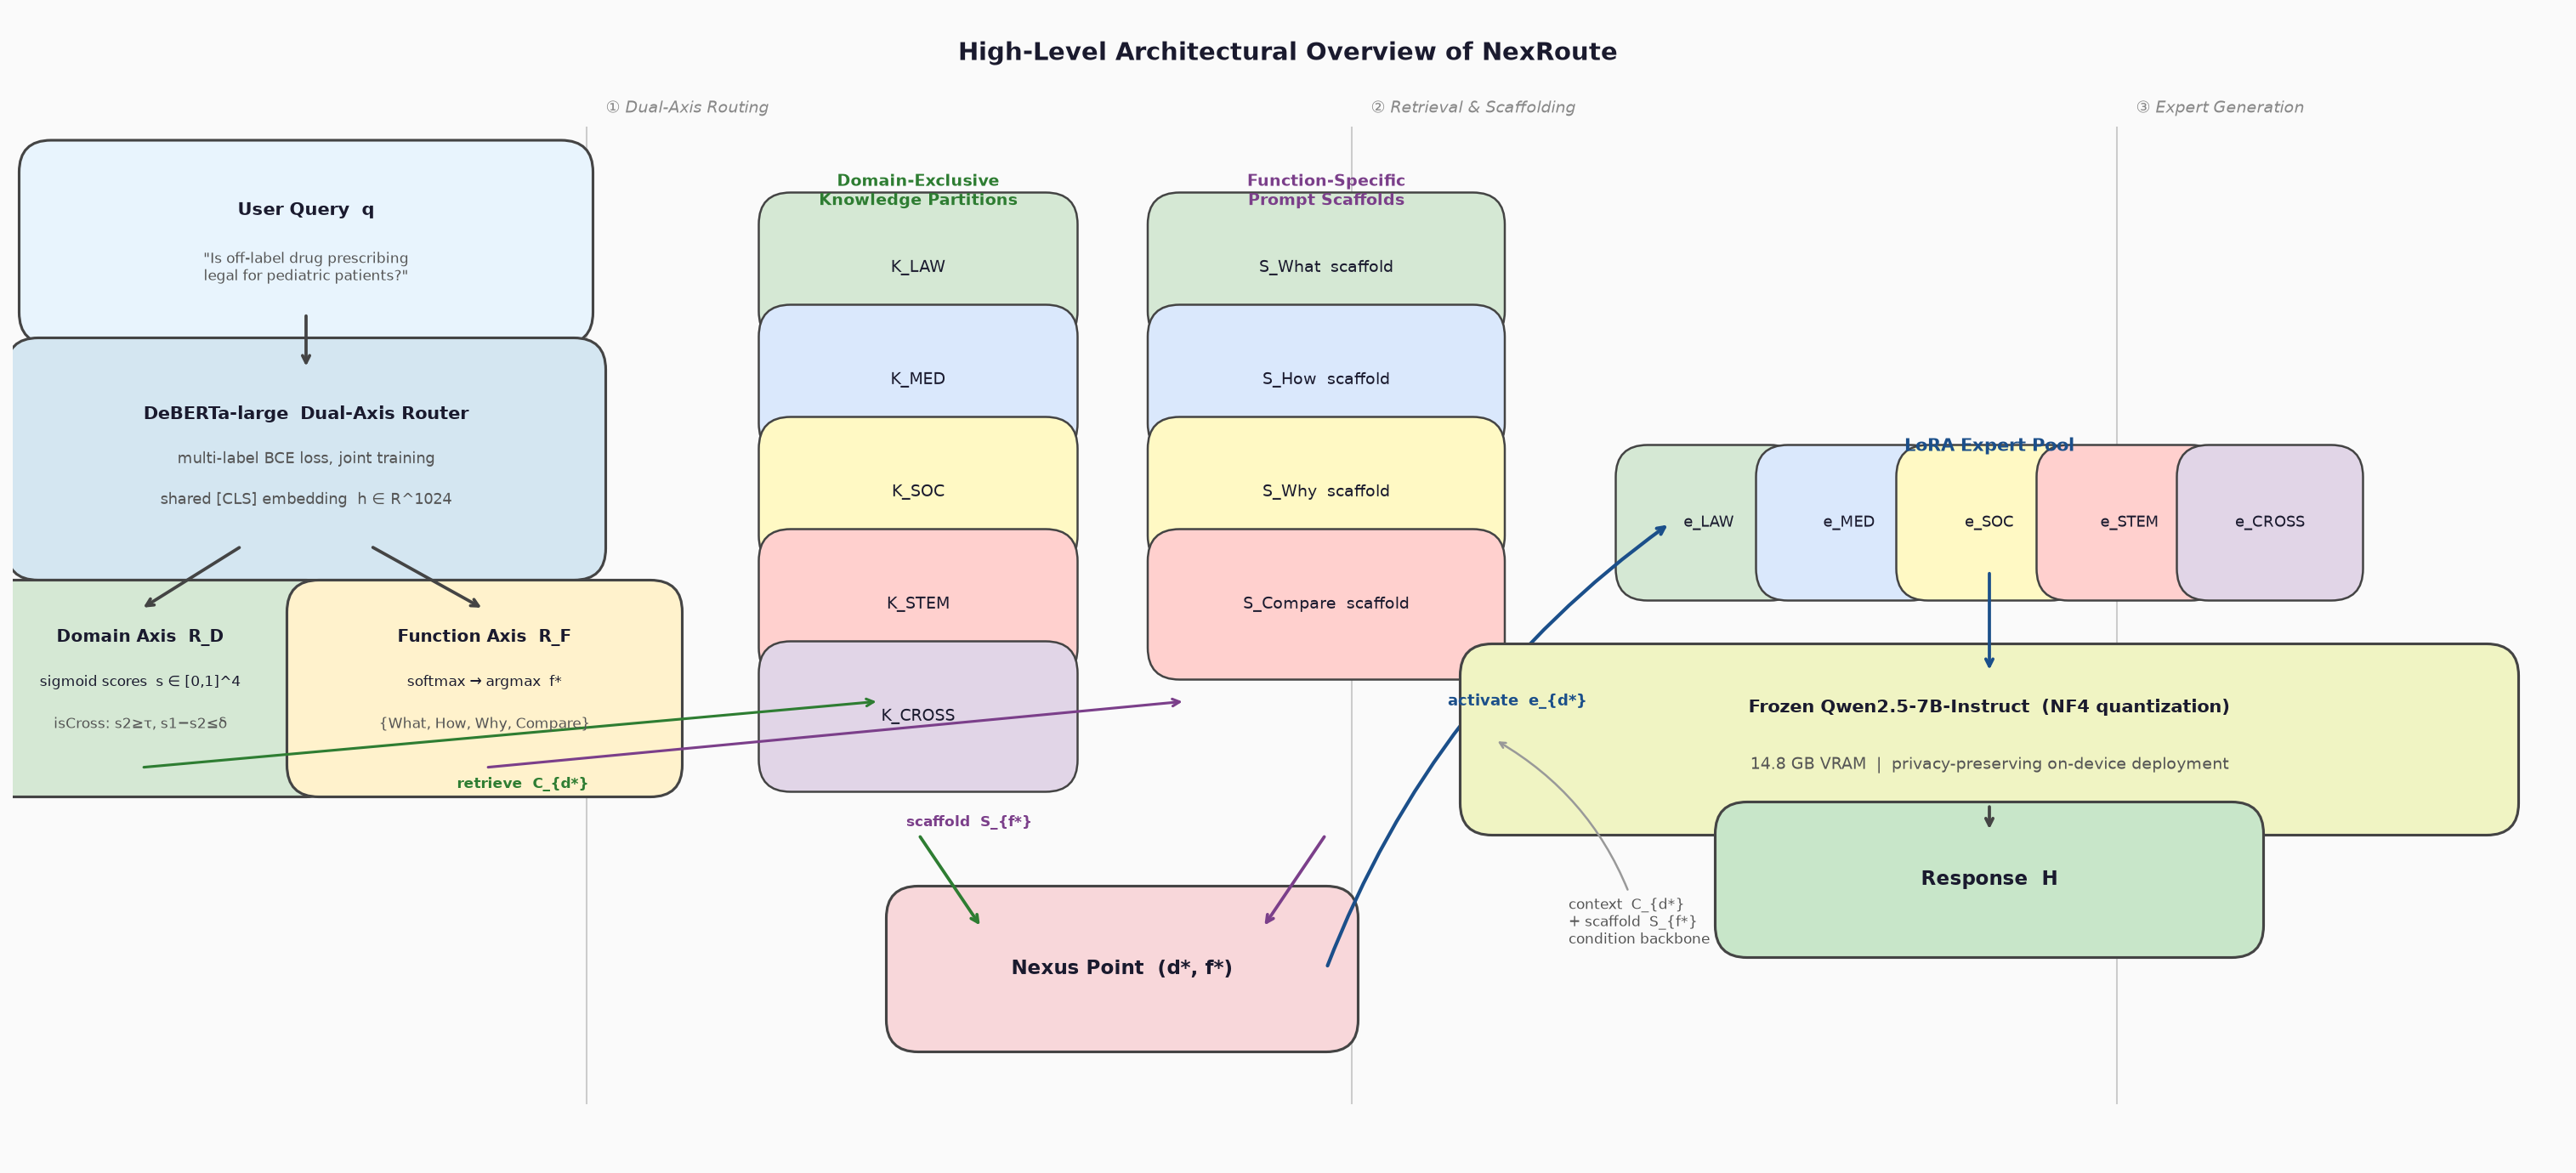
\includegraphics[width=\textwidth, height=0.85\textheight, keepaspectratio=true]{img11.png}
\end{center}
\begingroup
\captionof{figure}{High-level architectural overview of NexRoute. A user
query $q$ is jointly classified by the DeBERTa-large dual-axis router into
a domain score and a function label. The resulting nexus point determines
(1) the domain-exclusive retrieval partition (eliminating cross-domain
contamination by construction) and (2) the function-specific prompt scaffold,
which together condition the frozen Qwen2.5-7B-Instruct
backbone~\citep{qwen2025qwen25}. The corresponding LoRA adapter
($e_{\texttt{LAW}}$, $e_{\texttt{MED}}$, $e_{\texttt{SOC}}$,
$e_{\texttt{STEM}}$, or the dedicated $e_{\texttt{CROSS}}$ adapter when
\texttt{isCross}$(q){=}$\texttt{True}) is dynamically activated to generate
the final response.
(Inter-Domain Interference, IDI, is formally defined in
Section~\ref{ssec:retrieval}.)}
\label{fig:archoverview}
\endgroup
Let $q$ denote an input query. We define the \textbf{domain axis} as the
discrete set $\mathcal{D} = \{\texttt{LAW}, \texttt{MED}, \texttt{SOC}, \texttt{STEM}, \texttt{CROSS}\}$
and the \textbf{function axis} as
$\mathcal{F} = \{\texttt{What}, \texttt{How}, \texttt{Why}, \texttt{Compare}\}$.
NexRoute maintains domain-specialized LoRA adapters $\{e_d\}_{d \in \mathcal{D}}$
mounted on a shared frozen backbone. The routing problem is to identify the
\textit{nexus point} $(d^*, f^*)$ that jointly maximizes the posterior:
\begin{equation}
    (d^*, f^*) = \argmax_{d \in \mathcal{D},\, f \in \mathcal{F}} P(d, f \mid q).
    \label{eq:nexus_joint}
\end{equation}
We factorize as $P(d, f \mid q) = P(d \mid q) \cdot P(f \mid q)$ via a shared DeBERTa-large encoder ($\mathbf{h} \in \mathbb{R}^{1024}$), jointly training $R_D$ and $R_F$ under a composite loss (Eq.~\ref{eq:joint_loss}) for efficient multi-task disentanglement.
The inference pipeline proceeds in four synchronized stages
(Figure~\ref{fig:pipeline}):
\begin{enumerate}
    \item \textbf{Dual-axis routing}: $R_D$ and $R_F$ map $q$ to the nexus
    point $(d^*, f^*)$.
    \item \textbf{Domain-partitioned retrieval}: NexRoute queries exclusively
    the partition $\mathcal{K}_{d^*}$, fetching top-$K$ passages and
    eliminating cross-domain contamination by construction.
    \item \textbf{Function-aware prompt scaffolding}: The context
    $\mathcal{C}_{d^*}$ is restructured via scaffold $\mathcal{S}_{f^*}$,
    aligning the prompt with the required reasoning modality.
    \item \textbf{Expert-grounded generation}: The activated adapter $e_{d^*}$
    generates the final response conditioned on the function-structured context.
\end{enumerate}
%%------------------------------------------------------------------------------
\subsection{Domain-Partitioned Knowledge Base}
\label{ssec:retrieval}
%%------------------------------------------------------------------------------
\paragraph{Corpus construction.}
The full training corpus $\mathcal{K}$ is divided into five mutually exclusive
domain partitions satisfying strict offline exclusivity:
\begin{equation}
    \mathcal{K}_i \cap \mathcal{K}_j = \emptyset,
    \quad \forall i \neq j \in \mathcal{D}
    \label{eq:partition}
\end{equation}
We define \emph{Inter-Domain Interference} ($\mathrm{IDI}(q)$) as the
count of retrieved passages originating from a domain other than $d^*(q)$.
By Eq.~\ref{eq:partition}, domain-partitioned retrieval guarantees
$\mathrm{IDI}(q) = 0$ for all single-domain queries.

Each single-domain partition is built from MMLU benchmark
subsets~\citep{hendrycks2021mmlu}, with raw MCQ items rewritten into
open-ended instruction-answer pairs via Qwen2.5-72B-Instruct.
The 1,321 \texttt{CROSS} samples were synthesized to require joint causal
reasoning across domain pairs (e.g., MED$\times$LAW applying legal liability
doctrines to off-label pharmacology), verified via LLM-as-a-judge filtering
and a stratified human audit. Table~\ref{tab:cross_pairs_main} reports the
domain-pair distribution; full corpus statistics and quality-filtering details
are in Supplementary Material~S1.

\vspace{4pt}
\begin{center}
\begingroup
\renewcommand{\arraystretch}{1.3}
\captionof{table}{Domain-pair distribution of the \texttt{CROSS} partition
($n{=}1{,}321$). The \textsc{Law}--\textsc{Med} pair is \emph{absent} from
training, making it the held-out pair used in the case study
(Section~\ref{sec:casestudy}).}
\label{tab:cross_pairs_main}
\begin{tabular}{lrr}
\toprule
\textbf{Domain Pair} & \textbf{Count} & \textbf{Training?} \\
\midrule
MED--STEM  & 363 & \checkmark \\
LAW--SOC   & 527 & \checkmark \\
MED--SOC   & 298 & \checkmark \\
STEM--SOC  & 133 & \checkmark \\
\midrule
LAW--MED   &   0 & \textbf{Held-out} \\
\midrule
\textbf{Total} & \textbf{1,321} & \\
\bottomrule
\end{tabular}
\endgroup
\end{center}
\vspace{4pt}

%%------------------------------------------------------------------------------
\subsection{Dual-Axis Joint Router}
\label{ssec:domainrouter}
%%------------------------------------------------------------------------------
The domain axis router ($R_D$) and function axis classifier ($R_F$) share
a single pre-trained DeBERTa-large encoder---a bidirectional Transformer
built on BERT~\citep{devlin2019bert}---to map query $q$ into a contextualized
\texttt{[CLS]} representation $\mathbf{h} \in \mathbb{R}^{1024}$. This
shared representation branches into two independent classification heads.

\paragraph{Domain axis classification ($R_D$).}
$\mathbf{h}$ is passed through a two-layer MLP to produce domain scores:
\begin{equation}
    \hat{\mathbf{s}} = \sigma \left( W_2\, \text{ReLU}
    (W_1 \mathbf{h} + \mathbf{b}_1) + \mathbf{b}_2 \right) \in [0,1]^4
    \label{eq:router}
\end{equation}
where the four output scores correspond to the single-domain categories
$\{\texttt{LAW},\, \texttt{MED},\, \texttt{SOC},\, \texttt{STEM}\}$.
The \texttt{CROSS} label is \emph{not} a direct MLP output; it is instead
inferred from the joint activation pattern of the top-two single-domain
scores via the threshold criterion in Eq.~\ref{eq:cross_detect}, enabling
soft cross-domain detection without requiring an explicit fifth output neuron.

A query is classified as \texttt{CROSS} when the top-two domain scores
jointly satisfy both a minimum activation threshold $\tau$ and a maximum
score gap $\delta$:
\begin{equation}
    \text{isCross}(q) =
    \begin{cases}
        \texttt{True}  & \text{if } s_2 \geq \tau \;\text{and}\;
                         s_1 - s_2 \leq \delta \\
        \texttt{False} & \text{otherwise}
    \end{cases}
    \label{eq:cross_detect}
\end{equation}

Both hyperparameters were determined via grid search
($\tau \in [0.1, 0.5]$, $\delta \in [0.1, 0.6]$) on the validation set,
yielding a stable plateau ($<0.7$\%p variation). An asymmetric cost
criterion ($w_{\text{FN}}=3, w_{\text{FP}}=1$) selects
$\tau = 0.30$, $\delta = 0.40$, reducing \texttt{CROSS} false negatives
from 5.0\% to 3.0\% at a 3.7\%p increase in false-positive rate.
Table~\ref{tab:cross_fn_main} summarises the detection error trade-off between
the grid-search optimum and the adopted configuration. The full sensitivity
heatmap (Figure~S3.1) is in Supplementary Material~S3.

\vspace{4pt}
\begin{center}
\begingroup
\renewcommand{\arraystretch}{1.2}
\captionof{table}{\texttt{CROSS} detection error trade-off between grid-search
optimum and adopted configuration on the 500-sample held-out test set
($n_{\texttt{CROSS}}{=}100$, $n_{\text{single}}{=}400$). Val.\ Acc.\ is
binary \texttt{CROSS}-vs.-single detection; Test Acc.\ is full five-way
domain classification.}
\label{tab:cross_fn_main}
\begin{tabular}{lcccc}
\toprule
\textbf{Configuration} & \textbf{Val.\ Acc.} & \textbf{Test Acc.} & \textbf{FN Rate} & \textbf{FP Rate} \\
\midrule
$\tau$=0.50, $\delta$=0.10 (grid optimum) & 97.50\% & 88.60\% & 5.0\% & 4.5\% \\
$\tau$=0.30, $\delta$=0.40 (adopted)      & 97.20\% & 87.40\% & 3.0\% & 8.2\% \\
\bottomrule
\end{tabular}
\endgroup
\end{center}
\vspace{4pt}

\paragraph{Function axis classification ($R_F$).}
Simultaneously, $R_F$ determines the requisite reasoning strategy using a
softmax head over four mutually exclusive functional categories:
\begin{equation}
    \hat{\mathbf{p}} = \text{softmax}(W_F \mathbf{h} + \mathbf{b}_F)
    \in \mathbb{R}^4
    \label{eq:func}
\end{equation}
where $\hat{\mathbf{p}} = (\hat{p}_1, \hat{p}_2, \hat{p}_3, \hat{p}_4)$
corresponds to the four functional categories
$\{\texttt{What},\, \texttt{How},\, \texttt{Why},\, \texttt{Compare}\}$
respectively, and $f^* = \arg\max_k \hat{p}_k$.

\paragraph{End-to-End Joint Training.}
$R_D$ and $R_F$ are trained \emph{jointly} so that the shared encoder
$\mathbf{h}$ learns disentangled representations of domain membership and
reasoning function. The network is optimized via a composite loss function:
\begin{equation}
    \mathcal{L}_{\text{router}} = \lambda_D \mathcal{L}_{D}
    + \lambda_F \mathcal{L}_{F}
    \label{eq:joint_loss}
\end{equation}
where $\lambda_D = \lambda_F = 1.0$.
$\mathcal{L}_{D}$ is the \emph{binary} cross-entropy loss computed
independently for each of the four single-domain outputs, supporting
multi-label supervision. For a cross-domain sample spanning
\texttt{MED} and \texttt{LAW}, the target vector is
$\mathbf{y}_D = (1, 1, 0, 0)^\top$
(index order: \texttt{LAW}=1, \texttt{MED}=1, \texttt{SOC}=0,
\texttt{STEM}=0), enabling the router to assign high activation to both
contributing domains simultaneously. This dual-1 labelling allows
$R_D$ to detect cross-domain intent without requiring a dedicated
fifth output, as \texttt{CROSS} is inferred post-hoc via
Eq.~\ref{eq:cross_detect}.
$\mathcal{L}_{F}$ is the standard categorical cross-entropy loss for the functional intent label (training details in Table~\ref{tab:hyperparams_all}).

%%------------------------------------------------------------------------------
\subsection{Function-Aware Prompt Scaffolding}
\label{ssec:functionaxis}
%%------------------------------------------------------------------------------
The function axis structures retrieved context $\mathcal{C}_{d^*}$ through
a function-specific scaffold $\mathcal{S}_{f^*}$ that aligns the prompt with
the reasoning operation required by $q$. The final prompt is constructed as:
\begin{equation}
    \mathcal{P}(q, d^*, f^*) = \big[ \text{sys}_{d^*},\;
    \mathcal{S}_{f^*}(\mathcal{C}_{d^*}),\; q \big]
    \label{eq:prompt}
\end{equation}
where $\text{sys}_{d^*}$ is the domain-specific system instruction
(which incorporates a single domain-specific few-shot demonstration to
prime the expert's response format) and $\mathcal{S}_{f^*}$ is the
function-specific context scaffold (Table~\ref{tab:scaffolds}) that
dictates the reasoning pathway.

\vspace{4pt}
\begin{center}
\begingroup
\captionof{table}{Function-specific context scaffold templates $\mathcal{S}_{f^*}$.}
\label{tab:scaffolds}
\renewcommand{\arraystretch}{1.4}
\begin{tabular}{l p{9cm}}
\toprule
$f^*$ & \textbf{Scaffold Template} \\
\midrule
\texttt{What}
  & ``Based on the following evidence, identify and define the key facts.
    Do not infer beyond the provided context: \{context\}'' \\
\midrule
\texttt{How}
  & ``Using the following evidence, describe the mechanism or procedure
    in a step-by-step logical flow: \{context\}'' \\
\midrule
\texttt{Why}
  & ``Based on the following evidence, construct a definitive causal chain.
    Explicitly explain the underlying reasons connecting premise to
    outcome: \{context\}'' \\
\midrule
\texttt{Compare}
  & ``Using the following evidence, contrast the entities in the query.
    Highlight structural similarities and key differences in a comparative
    framework: \{context\}'' \\
\bottomrule
\end{tabular}
\endgroup
\end{center}
\vspace{4pt}

The four function categories, empirically validated with Cohen's $\kappa = 0.91$ and a hybrid exclusion rate below 3.2\%, are:

\begin{itemize}
    \item \textbf{What}: Factual extraction or definition (declarative recall).
    \item \textbf{How}: Step-by-step procedural or mechanistic explanation.
    \item \textbf{Why}: Causal or normative reasoning toward a conclusion.
    \item \textbf{Compare}: Contrastive analysis across entities or frameworks.
\end{itemize}


By aligning the prompt structure with the reasoning function $f^*$,
NexRoute ensures that the activated expert $e_{d^*}$ receives a reasoning
directive perfectly matched to its specialized parametric knowledge,
explicitly preventing functional mismatch at generation.
%%------------------------------------------------------------------------------
\subsection{Nexus-Point Expert Activation}
\label{ssec:nexus}
%%------------------------------------------------------------------------------
Given $(d^*, f^*)$, NexRoute dynamically loads the LoRA adapter $e_{d^*}$
onto the frozen backbone via PEFT's \texttt{load\_adapter} interface.
For single-domain queries:
\begin{equation}
    \mathbf{H} = \text{LLM}_{\theta + \Delta\theta_{d^*}} \big(
    \mathcal{P}(q, d^*, f^*) \big)
    \label{eq:single}
\end{equation}
where $\theta$ denotes the frozen Qwen2.5-7B-Instruct backbone and
$\Delta\theta_{d^*}$ the dynamically loaded adapter matrices.

For cross-domain queries (\texttt{isCross}$(q)$ = \texttt{True}), the
dedicated \texttt{CROSS} adapter is activated. The merged context
$\mathcal{C}_{\texttt{cross}}$ is constructed as the mathematically rigorous
union of the two independently retrieved sub-partitions:
\begin{equation}
    \mathcal{C}_{\texttt{cross}} = \mathcal{C}_{d_1} \cup \mathcal{C}_{d_2}
    \label{eq:cross_ctx}
\end{equation}
The final interdisciplinary response is generated as:
\begin{equation}
    \mathbf{H}_{\texttt{cross}} = \text{LLM}_{\theta +
    \Delta\theta_{\texttt{CROSS}}}
    \big( \mathcal{P}(q, \texttt{CROSS}, f^*) \big)
    \label{eq:cross_gen}
\end{equation}

%%------------------------------------------------------------------------------
\subsection{LoRA Expert Training and Quality Assurance}
\label{ssec:loratrain}
%%------------------------------------------------------------------------------
\paragraph{Adapter architecture.}
Following Hu et al.~\citep{hu2022lora}, we inject trainable low-rank matrices ($W' = W + \frac{\alpha}{r} BA$) into all linear modules (attention and feed-forward) across every Transformer layer to maximize expressivity. The Qwen2.5-7B backbone is frozen in 4-bit NormalFloat (NF4) quantization~\citep{dettmers2023qlora}, actively reducing VRAM footprint while cleanly isolating domain-specific updates within bfloat16 LoRA matrices.
\paragraph{Training configuration.}
Each expert is trained independently with autoregressive cross-entropy loss
and prompt masking; physical adapter isolation prevents negative transfer.
All hyperparameters are summarized in Table~\ref{tab:hyperparams_all}.
\paragraph{Data quality and bias mitigation.}
To train the function router ($R_F$), 15,744 items were annotated via a
two-stage pipeline: rule-based surface heuristics followed by a
Qwen2.5-72B-Instruct judge to capture implicit intents, excluding
unresolvable items. To mitigate circular-dependency bias from the Qwen
model family, three domain experts audited a 5\% sample ($n = 787$)
following a structured rubric. The audit yielded \textbf{94.2\%} agreement
(Cohen's $\kappa = 0.91$) via majority vote, validating the function-axis
annotations prior to training.

The dedicated $e_{\text{CROSS}}$ adapter is trained independently on 1,321
synthesized cross-domain samples to encode interdisciplinary reasoning
patterns; A direct comparison against weight-averaging and task-arithmetic weight-merging alternatives is left to future work (Section~7.2).

\begin{center}
\includegraphics[width=\textwidth, height=0.85\textheight, keepaspectratio=true]{img2.png}
\end{center}
\begingroup
\captionof{figure}{The NexRoute four-stage synchronized pipeline. An
incoming query $q$ is jointly classified by the Domain and Function axes.
Retrieval is restricted to the domain-exclusive partition
($\mathcal{K}_{d^*}$), ensuring $\mathrm{IDI}(q){=}0$
(Section~\ref{ssec:retrieval}). The fetched context is structurally
aligned via function-specific scaffolding ($\mathcal{S}_{f^*}$) before
generation by the activated LoRA expert ($e_{d^*}$).}
\label{fig:pipeline}
\endgroup
%%==============================================================================
\section{Experiments}
\label{sec:experiments}
%%==============================================================================

%%------------------------------------------------------------------------------
\subsection{Experimental Setup}
\label{ssec:setup}
%%------------------------------------------------------------------------------
\paragraph{Evaluation benchmark.}
We construct a held-out set of \textbf{500 samples} (100 per domain) drawn
from MMLU subsets corresponding to each domain partition; gold answers are
generated following the quality-control pipeline in Section~\ref{ssec:retrieval}.
The benchmark covers all five domain categories in $\mathcal{D}$.
Gold answers are produced by the same Qwen2.5-72B-Instruct model family
used for corpus construction (shared-lineage design); the shared-lineage
risk is quantified in Section~\ref{sec:limitations} via rank-correlation
analysis.
Primary factuality evaluation is reported in Section~\ref{sec:factuality}.

\paragraph{Baselines.}
We compare NexRoute against robust RAG baselines, all instantiated on the same
Qwen2.5-7B-Instruct backbone to ensure fair comparison:
\begin{itemize}
    \item \textbf{Naive RAG}: Standard dense retrieval over a unified knowledge
    base without domain routing or adapter specialization.

    \item \textbf{Adaptive RAG} \citep{jeong2024adaptiverag}: TF-IDF + LR
    keyword-based domain routing with unified retrieval, without LoRA
    specialization.

    \item \textbf{HyDE} \citep{gao2023hyde}: Hypothetical document embedding
    retrieval over a unified knowledge base.

    \item \textbf{CRAG} \citep{yan2024crag}: Corrective retrieval with
    quality-based re-retrieval over a unified knowledge base.
\end{itemize}
Additionally, we report the performance of massive dense models
(\textbf{Naive RAG 72B}, \textbf{Adaptive RAG 72B}, \textbf{HyDE 72B},
\textbf{CRAG 72B}; all Qwen2.5-72B-Instruct) to provide large-scale
reference points for parameter-scale comparison. LoRA-MoE variants
(e.g., LoRAMoE~\citep{dou2024loramoe}, Mixture-of-LoRAs~\citep{wu2024mixtureofloras})
are excluded from the main generation-quality comparison
(Table~\ref{tab:master_performance}; Supplementary Material~S5) as they are
designed for single-domain multi-task adaptation without cross-domain routing
mechanisms, rendering them architecturally incomparable to NexRoute's dual-axis
framework; they are referenced for routing-calibration context in
Section~\ref{ssec:router}, where applicable methodological details are provided.

\paragraph{Evaluation metrics.}
Text generation quality is measured using ROUGE-L \citep{lin2004rouge},
BERTScore \citep{zhang2020bertscore} with baseline rescaling, and BLEU-4
\citep{papineni2002bleu}. Routing performance is evaluated by exact-match
accuracy. Hallucination rate is measured via FActScore~\citep{min2023factscore} against the domain-partitioned knowledge base (union of both sub-partitions for CROSS queries).
Additional evaluation dimensions include computational efficiency (inference
latency and VRAM usage). Statistical
significance tests ($p < 0.05$) were performed via paired $t$-tests over the
500 evaluation samples.

%%------------------------------------------------------------------------------
\subsection{Routing System Accuracy}
\label{ssec:router}
%%------------------------------------------------------------------------------
Table~\ref{tab:router_acc} presents the domain routing accuracy of NexRoute
compared to Adaptive RAG, which serves as the strongest available routing
baseline. To ensure a strictly fair comparison and isolate the architectural
benefits of our dual-axis approach, the Adaptive RAG baseline was explicitly
trained on the identical \texttt{CROSS} class data, providing it the exact
same cross-domain supervision signal as NexRoute's DeBERTa router.

\vspace{6pt plus 4pt minus 3pt}
\begin{center}
\begingroup
\captionof{table}{Routing accuracy (exact match, \%) on 500 evaluation samples
($n{=}100$ per domain). $\Delta$ denotes percentage point improvement of
NexRoute over Adaptive RAG. Naive RAG, HyDE, and CRAG achieve 0\% routing
accuracy as they contain no routing mechanism. Adaptive RAG employs
TF-IDF$+$LR keyword-based routing; NexRoute employs a fine-tuned DeBERTa-large
dual-axis router.}
\label{tab:router_acc}
\begin{tabular}{lccr}
\toprule
\textbf{Domain} & \textbf{Adaptive RAG} & \textbf{NexRoute (Ours)} & \textbf{$\Delta$} \\
\midrule
LAW              & 92.0 & \textbf{99.0} & +7.0\%p \\
MED              & 84.0 & \textbf{85.0}  & +1.0\%p \\
SOC              & 68.0 & \textbf{76.0}  & +8.0\%p \\
STEM             & 87.0 & 80.0           & $-$7.0\%p \\
\midrule
CROSS            & 95.0 & \textbf{97.0}  & +2.0\%p \\
\midrule
\textbf{Total}   & 85.2 & \textbf{87.4}  & \textbf{+2.2\%p} \\
\bottomrule
\end{tabular}
\endgroup
\end{center}
\vspace{6pt plus 4pt minus 3pt}

\paragraph{Lexical overlap in adjacent domains.}
NexRoute achieves 87.4\% total routing accuracy, surpassing TF-IDF-based
Adaptive RAG by +2.2~pp. The largest gains occur in SOC (+8.0\%p) and LAW
(+7.0\%p), domains where keyword-based routing may be more susceptible to
surface-level lexical overlap. For instance, criminology-related sociological
queries share substantial vocabulary with legal statutes; this lexical
overlap is associated with higher misrouting rates in keyword-based systems.
NexRoute's DeBERTa-large router may better distinguish these adjacent domains
by attending to contextual semantics rather than surface word frequency,
though controlled ablations isolating this effect remain for future work.

\paragraph{STEM routing trade-off.}
STEM routing accuracy decreases by 7.0\%p (87.0\%$\to$80.0\%), a pattern
consistent with the widened \texttt{CROSS} activation margin ($\tau{=}0.30$,
$\delta{=}0.40$) increasing false positives on borderline STEM queries at
the cost of reduced false negatives on genuinely interdisciplinary queries.
The aggregate gains in SOC (+8.0\%p) and LAW (+7.0\%p) outweigh this
reduction at the total level (+2.2\%p; Table~\ref{tab:router_acc}), but for
users whose queries are predominantly STEM-domain, this configuration
represents a real accuracy cost. This design trade-off is discussed further in
Section~\ref{sec:discussion}.

\paragraph{Routing Error Analysis.}
To assess the generation-level impact of misrouted queries, we compare
generation quality between correctly routed ($n{=}437$) and misrouted
($n{=}63$) samples on the 500-sample evaluation set.
Table~\ref{tab:misrouted} reports the results.

\vspace{6pt plus 4pt minus 3pt}
\begin{center}
\begingroup
\captionof{table}{Generation quality for correctly routed vs.\ misrouted
samples under NexRoute 7B. Misrouted samples exhibit marginally higher
lexical scores, attributable to the majority (33/63) being
single$\to$\texttt{CROSS} misdirections that retrieve broader multi-domain
evidence from two domain partitions simultaneously.}
\label{tab:misrouted}
\begin{tabular}{lcccc}
\toprule
\textbf{Category} & \textbf{N} & \textbf{R-L} & \textbf{BS} & \textbf{B4} \\
\midrule
Correctly routed & 437 & 24.39 & 87.66 & 7.16 \\
Misrouted        &  63 & 26.87 & 88.78 & 8.99 \\
\bottomrule
\end{tabular}
\endgroup
\end{center}
\vspace{6pt plus 4pt minus 3pt}

Misrouted samples exhibit marginally higher generation quality across all
metrics. Of the 63 misrouted cases, 33 correspond to single-domain queries
misdirected to the \texttt{CROSS} expert (MED$\to$\texttt{CROSS}: 9;
SOC$\to$\texttt{CROSS}: 15; STEM$\to$\texttt{CROSS}: 9), which retrieve
evidence from two partitions
simultaneously. The broader retrieval context increases lexical overlap with
the gold reference. This indicates that even under incorrect routing to
\texttt{CROSS}, domain-partitioned retrieval preserves access to the primary
domain evidence, preventing quality degradation and confirming the robustness
of the retrieval architecture to moderate routing errors.

We note an important nuance in interpreting Table~\ref{tab:misrouted}: the
marginal quality advantage of misrouted samples does not imply that routing
accuracy is unimportant. Rather, it indicates that domain-partitioned retrieval
and function-aware scaffolding---not exact routing correctness per se---may
be important contributors to generation quality, with correct routing serving as the
mechanism that determines which evidence partition(s) are accessed. Under the
fail-safe threshold configuration, even ``incorrect'' routing to \texttt{CROSS}
preserves access to the primary domain partition, explaining why generation
quality remains robust to moderate routing errors. This reframes routing accuracy
as necessary for computational efficiency and retrieval precision, but not the
sole determinant of output quality.

\paragraph{Confusion Matrix Analysis.}
Figure~\ref{fig:confusion} visually corroborates this shift in the decision
landscape. The confusion matrices confirm that NexRoute's contextual
classification substantially reduces off-diagonal confusion between
SOC, MED, and LAW that plagued Adaptive RAG. Furthermore, the visible leakage
from STEM into CROSS in the right matrix is the direct, intended consequence
of our conservative thresholding, intentionally trading marginal single-domain 
precision for maximum cross-domain safety.

\begin{center}
\includegraphics[width=\textwidth, height=0.85\textheight, keepaspectratio=true]{figure4.png}
\end{center}
\begingroup
\captionof{figure}{Confusion matrices for Adaptive RAG (left) and NexRoute
(right) on 500 evaluation samples (100 per domain). NexRoute reduces
off-diagonal misclassification in SOC (+8.0\%p, 68.0\%$\to$76.0\%) and
LAW (+7.0\%p, 92.0\%$\to$99.0\%), where TF-IDF-based routing is most
susceptible to lexical overlap with adjacent domain terminology. STEM accuracy
decreases by $-$7.0\%p (87.0\%$\to$80.0\%), a direct consequence of the intentional 
fail-safe mechanism adopted to strictly minimize false negatives on critical 
interdisciplinary queries (Section~\ref{ssec:domainrouter}).}
\label{fig:confusion}
\endgroup

\paragraph{Router Calibration.}
To verify that routing decisions reflect genuine distributional uncertainty,
we compute the Shannon entropy $H$ of each router's output over
\texttt{CROSS}-domain queries. NexRoute's router yields $H{=}0.667$~nats
(48.1\% of $H_{\max}{=}1.386$~nats for a 4-class distribution), correctly
reflecting cross-domain ambiguity. By contrast, re-implemented LoRAMoE-style
and Mixture-of-LoRAs routers yield normalized \texttt{CROSS}-query entropies
of only 3.8\% and 1.0\% of $H_{\max}$ respectively---committing to a single
domain with high confidence even on genuinely interdisciplinary queries, which
is consistent with their lower routing accuracy (78.0\% and 79.6\% vs.\
NexRoute's 87.4\%). A representative lexical-imbalance failure-mode analysis
is provided in Supplementary Material~S6.

%%------------------------------------------------------------------------------
\subsection{Comprehensive Generation Quality and System Efficiency}
\label{ssec:comprehensive}
%%------------------------------------------------------------------------------
Table~\ref{tab:master_performance} presents generation quality and computational efficiency across all baselines at 7B and 72B scales, averaged over three seeds (NexRoute 7B: std\ $<0.8$; 72B-scale models: std\ $<0.4$).

\vspace{6pt plus 4pt minus 3pt}
\begin{center}
\begingroup
\captionof{table}{Comprehensive performance profile of NexRoute compared to
RAG baselines. Generation metrics are reported separately for CROSS-domain
($n{=}100$) and Single-domain ($n{=}400$; $n{=}390$ for CRAG~7B,
MED$+$SOC$+$STEM$+$LAW) queries.
BERTScore is computed using \texttt{roberta-large} without baseline
rescaling~\citep{zhang2020bertscore}.
$\dagger$~CRAG~7B evaluated on 490 samples (10 STEM-domain generation
timeouts excluded; see Supplementary Material~S5).
$*$~NexRoute 7B CROSS-domain results are statistically significant over all
72B-scale dense baselines ($p < 0.05$, paired $t$-test, $n{=}500$).
Standard deviations across the three seeds are omitted from the table for
space; aggregate variance is reported in the text
(NexRoute 7B: std $<0.8$; 72B-scale models: std $<0.4$).}
\label{tab:master_performance}
\resizebox{\textwidth}{!}{%
\begin{tabular}{lcccccc}
\toprule
\multirow{2}{*}{\textbf{Model}}
  & \multicolumn{3}{c}{\textbf{CROSS-Domain Quality}}
  & \multicolumn{3}{c}{\textbf{Single-Domain Quality}} \\
\cmidrule(lr){2-4} \cmidrule(lr){5-7}
  & \textbf{ROUGE-L} & \textbf{BERTScore} & \textbf{BLEU-4}
  & \textbf{ROUGE-L} & \textbf{BERTScore} & \textbf{BLEU-4} \\
\midrule
\multicolumn{7}{l}{\textit{7B Parameter Scale Models:}} \\
Naive RAG 7B
  & 24.95 & 88.64 & 9.57
  & 25.56 & 88.14 & 9.15 \\
Adaptive RAG 7B
  & 24.25 & 88.44 & 8.92
  & 25.04 & 88.08 & 8.86 \\
HyDE 7B
  & 24.57 & 88.64 & 9.38
  & 25.36 & 88.14 & 9.15 \\
CRAG 7B$^\dagger$
  & 21.63 & 88.02 & 7.39
  & 25.28 & 88.15 & 9.05 \\
\textbf{NexRoute 7B (Ours)}
  & \textbf{29.60}$^{*}$ & \textbf{89.53}$^{*}$ & \textbf{10.75}
  & 24.02 & 87.37 & 8.12 \\
\midrule
\multicolumn{7}{l}{\textit{72B Parameter Scale Models (Large-Scale Reference):}} \\
Naive RAG 72B
  & 28.81 & 89.03 & 13.27
  & \textbf{30.85} & 89.06 & 12.96 \\
Adaptive RAG 72B
  & 28.54 & 89.07 & 13.02
  & 30.25 & 88.99 & 12.57 \\
HyDE 72B
  & 28.61 & 89.02 & 13.24
  & 30.38 & 88.97 & 12.87 \\
CRAG 72B
  & 28.95 & 89.10 & 13.22
  & 30.22 & 88.97 & 12.79 \\
\textbf{NexRoute 72B (Ours)}
  & \textbf{30.76} & \textbf{90.96} & \textbf{13.64}
  & 30.80 & \textbf{89.08} & \textbf{13.34} \\
\bottomrule
\end{tabular}%
}
\endgroup
\end{center}
\vspace{6pt plus 4pt minus 3pt}

\paragraph{Cross-domain performance: NexRoute 7B vs.\ 72B baselines.}
NexRoute 7B leads all 7B baselines and surpasses all 72B-scale dense baselines on CROSS-domain ROUGE-L and BERTScore ($p{<}0.05$, paired $t$-test; Table~\ref{tab:master_performance}). This result at $10{\times}$ fewer parameters suggests that structural specialization---domain-partitioned retrieval combined with function-aware scaffolding---may partially substitute for raw parameter scale in cross-domain generation settings, though confirmation across broader evaluation conditions is required. The BLEU-4 gap vs.\ CRAG 72B may partly reflect function-scaffolded output conciseness rather than semantic deficiency (see Section~\ref{sssec:causal-density}), though we note that BLEU-4 can be sensitive to both response length and $n$-gram overlap characteristics.
Figure~\ref{fig:performance} visualizes these results across model scales.

\begin{center}
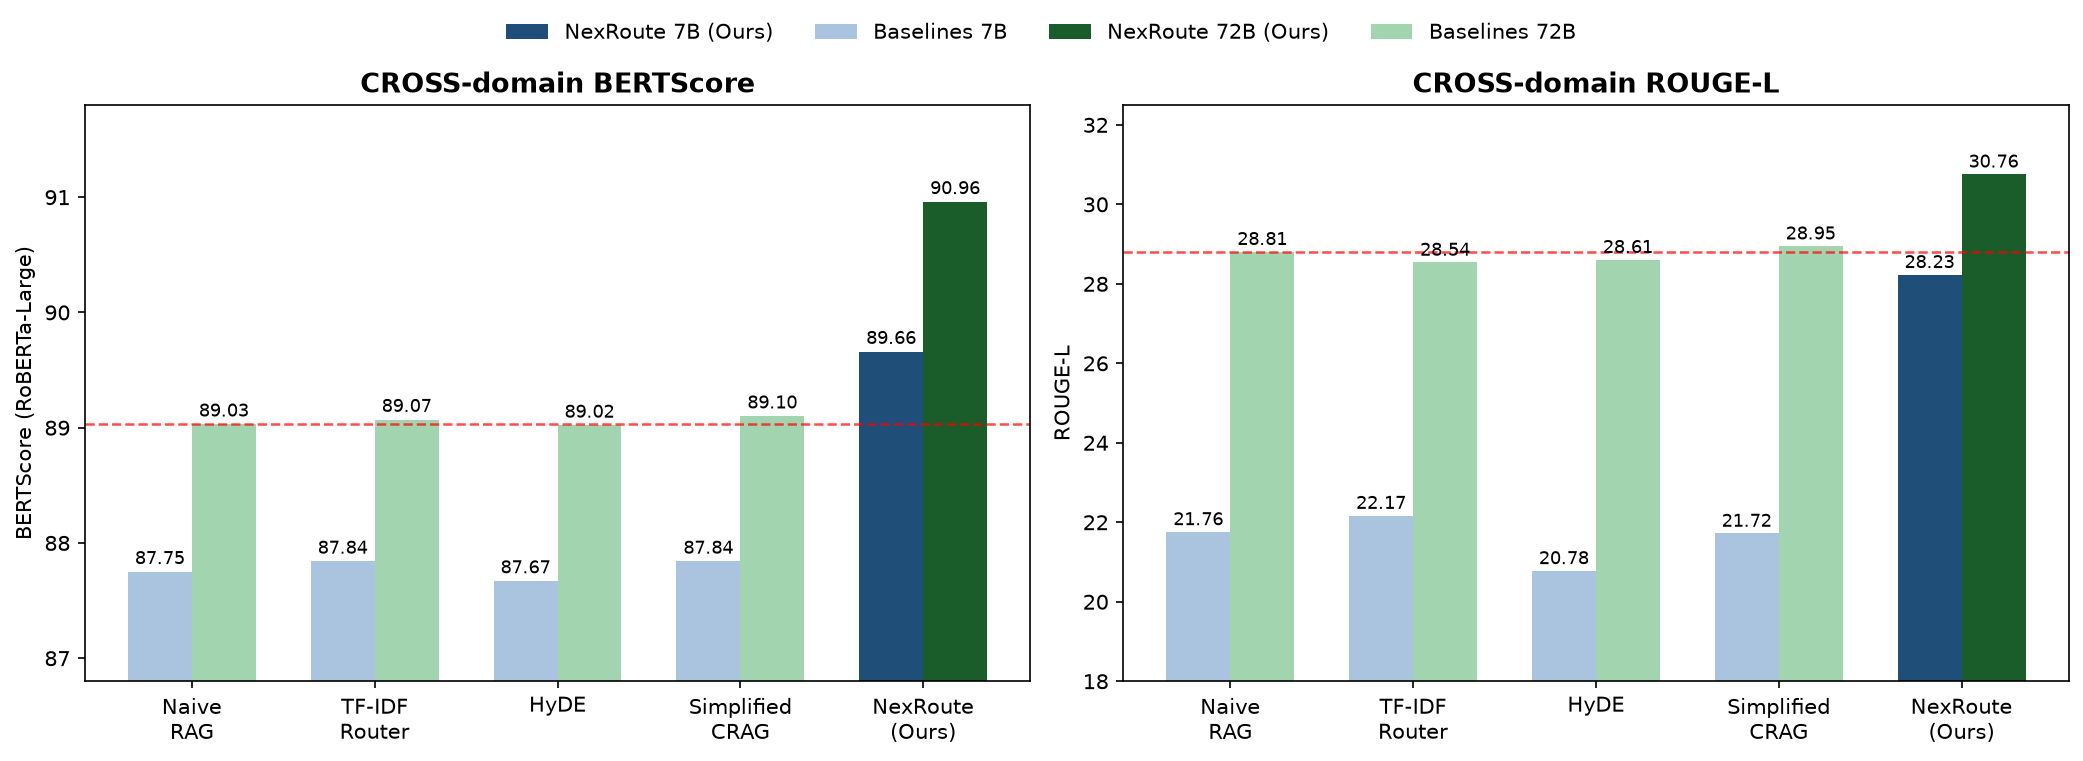
\includegraphics[width=\textwidth, height=0.85\textheight, keepaspectratio=true]{figure5.png}
\end{center}
\begingroup
\captionof{figure}{CROSS-domain generation quality (BERTScore, ROUGE-L)
across 7B and 72B model scales. NexRoute 7B leads all 7B baselines on
ROUGE-L and BERTScore, and surpasses all 72B-scale dense baselines,
suggesting that architectural specialization can compensate for parameter
scale on these cross-domain tasks (see caveat in text).}
\label{fig:performance}
\endgroup

\paragraph{Per-domain performance.}
NexRoute 7B leads in MED (ROUGE-L 25.78, BLEU-4 10.78) and SOC (BERTScore 88.37), where domain-partitioned specialization provides a measurable advantage. STEM and LAW are competitive with unified-retrieval baselines. Full per-domain breakdowns for all models and scales are in Supplementary Material~S5.

\paragraph{Single-domain trade-off.}
NexRoute 7B's aggregate single-domain ROUGE-L (24.02) trails Naive RAG 7B (25.56), a structurally expected cost of domain-partitioned LoRA specialization that is outweighed by the CROSS-domain gains (full per-domain breakdown in Supplementary Material~S5).

\paragraph{Computational efficiency and deployment feasibility.}
NexRoute 7B's dynamic adapter switching maintains peak VRAM usage at
\textbf{14.8~GB}, fitting within commodity hardware (e.g., RTX~4090).
72B-scale baselines require approximately 36--40~GB of VRAM and incur
substantially higher inference latency (full profile in Supplementary Material~S2).

\paragraph{Factuality and hallucination rate.}
NexRoute 7B achieves the lowest overall hallucination rate of \textbf{8.9\%}
among 7B-scale models---a reduction of 1.7~pp from Naive RAG 7B (10.6\%;
$p{=}0.075$, $h{=}0.06$), 3.2~pp from Adaptive RAG (12.1\%; $p{=}0.001$,
$h{=}0.11$), and 2.2~pp from CRAG (11.1\%; $p{=}0.026$, $h{=}0.08$)
(Table~\ref{tab:hallucination}). Effect sizes are small ($h{<}0.2$) across
all comparisons. Domain-partitioned retrieval, by restricting evidence to
domain-exclusive passages, may reduce the introduction of domain-incongruent
claims associated with unified retrieval; however, the $p{=}0.075$ result for
the Naive RAG comparison indicates that this specific pairwise difference
should be interpreted cautiously. NexRoute 7B's CROSS-domain hallucination
rate (4.3\%) is tied with Naive RAG 7B (4.3\%) as the lowest among all
evaluated models, while its overall rate (8.9\%) is the lowest across all
7B baselines.
Figure~\ref{fig:hallucination} illustrates the hallucination suppression effect.

\begin{center}
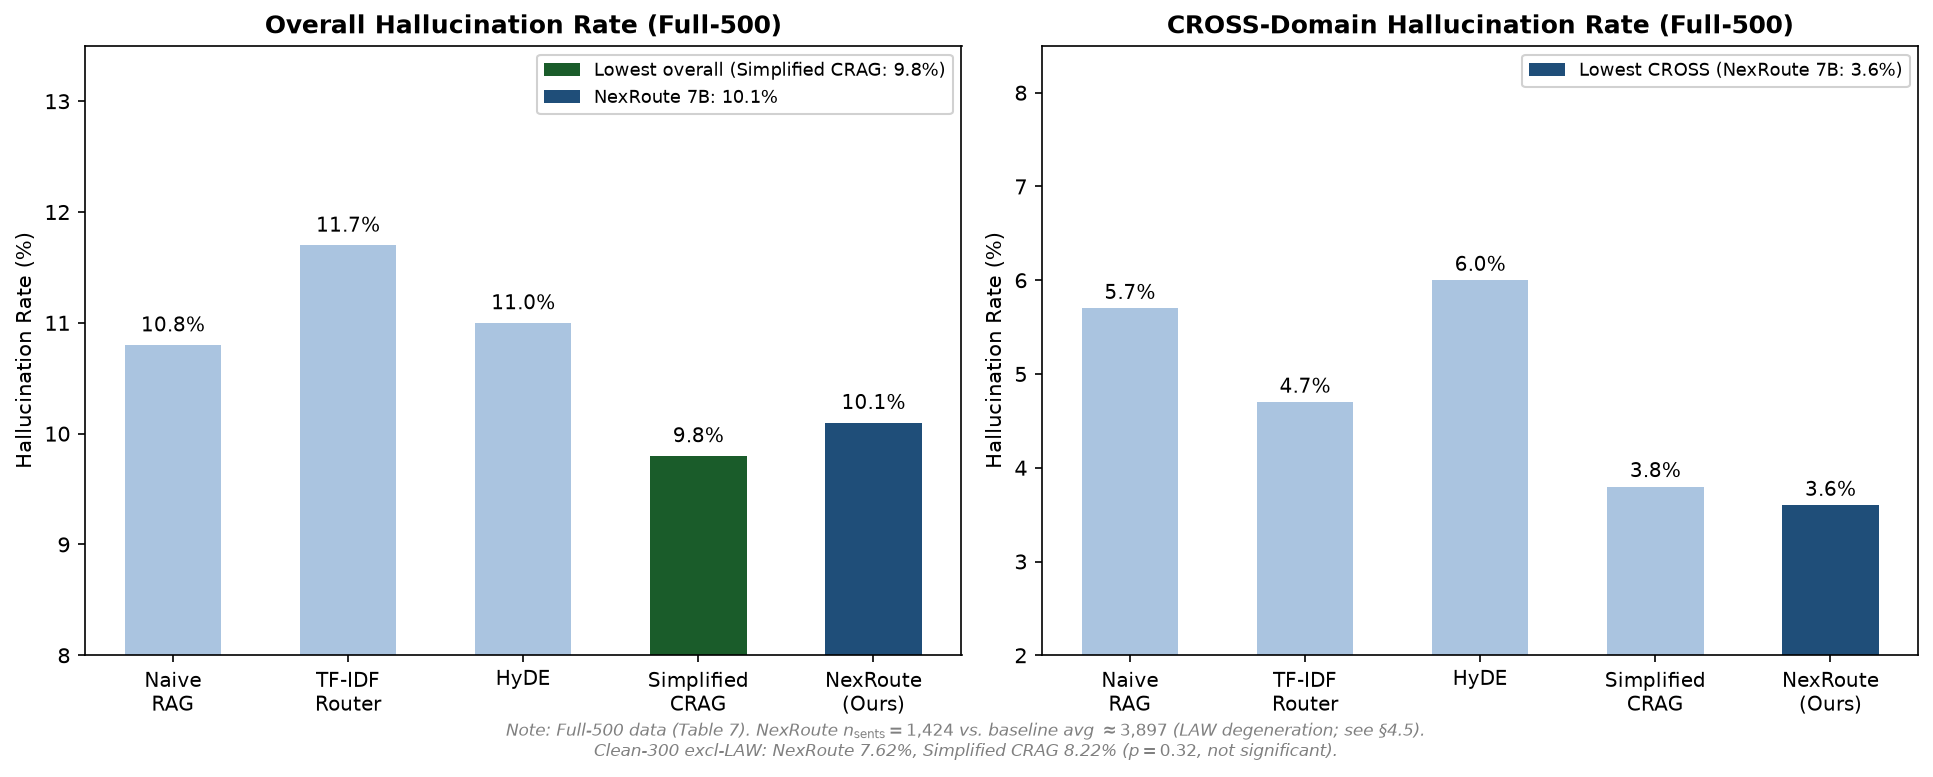
\includegraphics[width=\textwidth, height=0.85\textheight, keepaspectratio=true]{figure6.png}
\end{center}
\begingroup
\captionof{figure}{Impact of domain-partitioned retrieval on hallucination
rate. (Left) Hallucination rates across all 7B baselines; NexRoute 7B
achieves the lowest overall rate of 8.9\% (16.0\% relative reduction vs.\
Naive RAG 7B at 10.6\%), measured via domain-aligned FActScore. (Right)
Direct comparison of systems with and without domain-partitioned retrieval,
consistent with partition-exclusive retrieval being an important contributor
to hallucination suppression in this evaluation.}
\label{fig:hallucination}
\endgroup

%%------------------------------------------------------------------------------
\subsection{Factuality Assessment}
\label{sec:factuality}
%%------------------------------------------------------------------------------
\vspace{6pt plus 4pt minus 3pt}
\begin{center}
\begingroup
\captionof{table}{Hallucination rates (\%) evaluated via FActScore across
7B-backbone models. Lower hallucination rate is better.
\textit{Relative Reduction} is computed against Naive RAG as the
reference baseline. Superscript $\ddagger$ indicates a statistically
significant difference from Naive RAG ($p < 0.05$, sentence-level
$\chi^2$ test); effect sizes (Cohen's $h$) are small ($h < 0.2$).
$\dagger$~CRAG CROSS subset evaluated on $n{=}100$ items (see Table~\ref{tab:master_performance} footnote).
$p$: unadjusted two-sided $p$-value (NexRoute vs.\ each model; sentence-level
$\chi^2$). $q$: Benjamini-Hochberg adjusted $p$-value within the
three-comparison family (NexRoute vs.\ Naive~RAG, Adaptive~RAG, CRAG;
$\alpha{=}0.05$). HyDE not tested against NexRoute.}
\label{tab:hallucination}
\begin{tabular}{lcccc cc}
\toprule
\textbf{Model} & \textbf{Overall (\%)} & \textbf{CROSS (\%)} & \textbf{Single (\%)} & \textbf{Rel. Reduction} & $p$ & $q$ \\
\midrule
Naive RAG       & 10.6 & 4.3 & 12.6 & ---                & 0.075 & 0.075 \\
Adaptive RAG    & 12.1 & 6.4 & 13.9 & $-14.2\%^\ddagger$ & 0.001 & 0.003 \\
HyDE            &  9.8 & 4.8 & 11.4 & $+7.5\%$           & ---   & ---   \\
CRAG$^\dagger$  & 11.1 & 5.6 & 12.1 & $-4.7\%$           & 0.026 & 0.039 \\
\textbf{NexRoute (Ours)} & \textbf{8.9} & \textbf{4.3} & \textbf{11.7} & $\mathbf{+16.0\%}$ & --- & --- \\
\bottomrule
\end{tabular}
\endgroup
\end{center}
\vspace{6pt plus 4pt minus 3pt}

\vspace{6pt plus 4pt minus 3pt}
\begin{center}
\begingroup
\captionof{table}{Ablation study: hallucination rates (\%) for NexRoute component
variants, evaluated via FActScore on CROSS-domain queries.
$\Delta$Overall and $\Delta$CROSS are percentage-point differences
relative to V01 (full NexRoute); positive values indicate \textit{more}
hallucination.
Superscripts denote BH-adjusted $q$-values within the four-comparison family
(V02--V03 $\times$ CROSS/Single subsets; sentence-level $\chi^2$):
$^{**}q < 0.01$; V03 CROSS: $q{=}0.19$ (non-significant, no superscript).
Cohen's $h{=}0.195$ (V01 vs.\ V02 Overall).
$^\S$~V04 and V05 generate responses 3.7$\times$ and 4.0$\times$ longer
than V01; hallucination rates may be partially attributable to response
length; these variants were not formally tested (effects ${\leq}1.6$\,pp).
V06 (Dominant-Single CROSS merging) results are in Supplementary Material~S4.}
\label{tab:ablation}
\begin{tabular}{lcccccc}
\toprule
\textbf{Variant} & \textbf{Overall} & \textbf{CROSS} & \textbf{Single} & $\boldsymbol{\Delta}$\textbf{Overall} & $\boldsymbol{\Delta}$\textbf{CROSS} & $\boldsymbol{\Delta}$\textbf{Single} \\
\midrule
V01 Full NexRoute (Ours)       &  8.9 & 4.3 & 11.7 & ---    & ---              & ---              \\
V02 w/o Function Axis          & 15.2 & 9.1 & 18.4 & $+6.3$ & $+4.8^{**}$      & $+6.7^{**}$      \\
V03 w/o Partitioned Retrieval  & 12.1 & 6.1 & 16.7 & $+3.2$ & $+1.8$           & $+5.0^{**}$      \\
V04 w/o LoRA                   &  9.3 & 5.4 & 10.8 & $+0.4$ & $+1.1^\S$        & $-0.9^\S$        \\
V05 w/o Domain Axis            & 10.5 & 6.5 & 12.2 & $+1.6$ & $+2.2^\S$        & $+0.5^\S$        \\
\midrule
\end{tabular}
\endgroup
\end{center}
\vspace{6pt plus 4pt minus 3pt}

Table~\ref{tab:hallucination} presents hallucination rates (FActScore) for all 7B models.
NexRoute achieves the lowest overall hallucination rate of 8.9\%---a 16.0\%
relative reduction compared to Naive RAG (10.6\%).
This reduction is statistically significant relative to Adaptive RAG
($p{=}0.001$) and CRAG ($p{=}0.026$), and represents a consistent trend
relative to Naive RAG ($p{=}0.075$), though the latter does not reach
conventional significance at $\alpha{=}0.05$.
To account for multiple comparisons across the three pairwise tests, we
additionally report Benjamini-Hochberg adjusted $q$-values
(Table~\ref{tab:hallucination}); both significant results
(Adaptive~RAG: $q{=}0.003$; CRAG: $q{=}0.039$) remain significant after
correction ($q{<}0.05$), while the Naive~RAG comparison remains
non-significant ($q{=}0.075$).
Domain-level breakdown reveals that NexRoute's advantage spans both evaluation
subsets: the CROSS-domain hallucination rate is 4.3\%---tied with Naive RAG
as the lowest among all models---while the single-domain rate is 11.7\%,
below all other 7B baselines (Naive RAG: 12.6\%).
Adaptive RAG and CRAG exhibit overall hallucination rates above Naive RAG
(12.1\% and 11.1\%, respectively), suggesting that their adaptive retrieval
heuristics introduce additional factual noise without corresponding accuracy
gains in this multi-domain setting.

The ablation study (Table~\ref{tab:ablation}) identifies the
\textbf{Function Axis} as the dominant structural contributor to factuality.
Removing the Function Axis (V02) increases overall hallucination from 8.9\%
to 15.2\% ($+$6.3\,pp; $p{<}0.001$), with significant degradation in both
CROSS ($+$4.8\,pp; $p{=}0.003$) and single-domain ($+$6.7\,pp; $p{<}0.001$)
subsets.
The Function Axis partitions inference responsibility among LoRA-based domain
experts via function-typed routing; its removal forces all queries through a
single generalist pathway, substantially increasing the rate of unverified
claims.
Removing Partitioned Retrieval (V03) raises single-domain hallucination by
5.0\,pp (11.7\%$\to$16.7\%; $p{=}0.003$, $h{=}0.16$), while the CROSS-domain
increase is smaller ($+$1.8\,pp; $p{=}0.19$), consistent with CROSS queries
distributing retrieval load across multiple partitions.
Applying Benjamini-Hochberg correction to the four sub-comparisons (V02 and
V03 across CROSS and Single subsets) leaves all conclusions unchanged: V02
and V03 Single remain significant ($q{<}0.01$), while V03 CROSS remains
non-significant ($q{=}0.19$; Table~\ref{tab:ablation}).
V06 (Dominant-Single CROSS merging) and extended V03 analysis are detailed
in Supplementary Material~S4.

Weight-averaging and task-arithmetic CROSS adapter variants were excluded from FActScore comparison due to insufficient atomic claim counts ($n$=319 and $n$=127 sentences, respectively) for reliable hallucination estimation; a full quantitative comparison including ROUGE-L, BERTScore, and BLEU-4 for these variants is left to future work (Section~7.2).

%%==============================================================================
\section{Case Study: Medical-Legal Dispute Analysis}
\label{sec:casestudy}
%%==============================================================================
We examine a complex medical-legal query to illustrate the specific reasoning mechanisms that drive NexRoute's aggregate results. \emph{The analyses in this section are qualitative and based on a single held-out instance; they are intended to be illustrative of architectural mechanisms rather than statistically conclusive, and all patterns should be interpreted with this scope in mind.}

%%------------------------------------------------------------------------------
\subsection{Scenario Definition}
\label{ssec:scenario}
%%------------------------------------------------------------------------------
We construct a representative cross-domain query spanning the \textsc{Medical}
and \textsc{Legal} knowledge domains. The \textsc{Law}--\textsc{Med} domain
pair is \emph{not} among the four pairs on which the \texttt{CROSS} adapter
was trained (Table~\ref{tab:cross_pairs_main}); this scenario therefore
constitutes a held-out evaluation probing generalization beyond the training
distribution. All qualitative findings below should be interpreted with this
limitation in mind:
\vspace{4pt}
\begin{tcolorbox}[colback=gray!8, colframe=gray!40, arc=2pt,
  boxrule=0.5pt, left=6pt, right=6pt, top=4pt, bottom=4pt]
\small\itshape
A patient suffered from severe hepatotoxicity after being prescribed Drug X
for weight loss. The doctor obtained a general treatment consent form but did
not specifically warn about liver damage, as weight loss is an off-label use
for Drug X. \textbf{Why} might the physician be held legally liable despite
the signed consent form?
\end{tcolorbox}
\vspace{4pt}
\noindent
This query is classified as $d^* = \texttt{CROSS}$ (\textsc{Law} $\oplus$
\textsc{Med}) and $f^* = \texttt{Why}$, requiring causal reasoning that bridges
\textit{pharmacological} evidence (the hepatotoxicity mechanism of Drug X) with
\textit{legal doctrine} (the duty of specific disclosure under off-label
informed consent law). This combination constitutes an ideal stress-test: a
system must simultaneously retrieve domain-partitioned evidence \emph{and}
apply a causal reasoning strategy to synthesize it---any failure in either
dimension collapses to surface-level enumeration of disconnected facts.

%%------------------------------------------------------------------------------
\subsection{Internal Pipeline Execution}
\label{ssec:pipeline}
%%------------------------------------------------------------------------------
All systems share the same \texttt{Qwen2.5-7B-Instruct} backbone with
top-$K{=}10$ dense retrieval, with the exception of the 72B-scale baselines
which share the corresponding \texttt{Qwen2.5-72B-Instruct} backbone under
identical retrieval settings. The key architectural differences lie in how
each system structures its retrieval scope and generation prompt.

The three unified-retrieval baselines (Naive RAG, HyDE, CRAG) all retrieve
from a single merged knowledge base, differing only in retrieval strategy:
Naive RAG uses direct query embedding; HyDE first generates a hypothetical
answer to improve retrieval precision; CRAG applies self-evaluated re-retrieval
when initial passages score below a relevance threshold. Critically, none of
these systems applies domain partitioning or function-aware prompting,
leaving the causal synthesis entirely to the model without structural support.
Adaptive RAG applies keyword-based domain routing but without LoRA
specialization or functional scaffolding, providing partial domain separation
at the cost of semantic precision.

NexRoute processes the query as follows:
\begin{enumerate}
    \item \textbf{Dual-Axis Routing.} The DeBERTa-large router
    ($\tau{=}0.30$, $\delta{=}0.40$) detects competing signals from clinical
    terms (\textit{hepatotoxicity}, \textit{Drug X}) and legal terms
    (\textit{liable}, \textit{consent form}), triggering the cross-domain
    criterion (Eq.~\ref{eq:cross_detect}) and setting $d^* = \texttt{CROSS}$
    (\textsc{Law}$+$\textsc{Med}). Simultaneously, $R_F$ identifies the causal
    interrogative (\textit{``Why might\ldots''}) and sets
    $f^* = \texttt{Why}$.

    \item \textbf{Domain-Partitioned Retrieval.} The retrieval budget is
    allocated proportionally to domain confidence scores
    (proportional budget allocation described in Supplementary Material~S1),
    independently fetching passages from the
    \textsc{Law} partition (malpractice case law, informed consent doctrine)
    and the \textsc{Med} partition (hepatotoxicity registries, off-label
    pharmacology), eliminating inter-domain contamination by construction.

    \item \textbf{Function-Aware Prompt Scaffolding.} The \texttt{Why}-scaffold
    structures the retrieved context into a three-stage causal reasoning
    directive: (1)~the pharmacological mechanism involved, (2)~the legal causal
    chain connecting the omission to liability, and (3)~the broader normative
    implication.

    \item \textbf{Expert-Grounded Generation.} The dedicated \texttt{CROSS}
    LoRA adapter generates the final response conditioned on the
    function-structured, domain-partitioned prompt.
\end{enumerate}

%%------------------------------------------------------------------------------
\subsection{Output Comparison and Analysis}
\label{ssec:output}
%%------------------------------------------------------------------------------
The fundamental challenge of this query lies in the requirement to
\emph{simultaneously} apply pharmacological knowledge (the specific
hepatotoxicity risk profile of Drug X under off-label metabolic pathways) and
legal doctrine (the informed consent obligation that shifts when a drug is
prescribed outside its approved indication). A system that retrieves only
medical evidence will accurately characterize the risk but fail to establish
legal liability; a system that retrieves only legal evidence will cite the
informed consent doctrine but lack the clinical specificity to connect the
omitted warning to the actual harm. A system that retrieves and integrates both evidence streams---with causal
structure preserved---may be better positioned to produce a legally and
medically coherent response.

NexRoute 7B produced the following response (78 tokens, shortest among all five 7B systems):
\begin{quote}\small
\textit{``The physician may be held liable due to a breach of the \textbf{specific duty of disclosure} inherent in off-label prescriptions. While a general consent form covers standard procedural risks, off-label use (e.g., Drug X for weight loss) shifts the legal burden. The physician must explicitly disclose unapproved, severe risks like hepatotoxicity to satisfy the requirements of \textbf{informed consent}. Because this specialized warning was omitted, the general consent form is legally invalidated regarding this specific complication.''}
\end{quote}
In contrast, Naive RAG 72B---despite $10\times$ the parameter count---enumerated medical facts and legal concepts in sequence without causal synthesis, implicitly validating the signed consent form as sufficient legal protection and entirely missing the off-label disclosure obligation. Verbatim outputs for all 7B and 72B systems, together with detailed failure-mode analyses, are in Supplementary Material~S7.

%%------------------------------------------------------------------------------
\subsubsection{NexRoute's Architectural Advantages}
\label{sssec:nexroute-advantages}
%%------------------------------------------------------------------------------

\paragraph{NexRoute 7B (Ours).}
As noted in Section~\ref{ssec:scenario}, this query instantiates the held-out
\textsc{Law}--\textsc{Med} domain pair absent from \texttt{CROSS} adapter
training; the following analysis constitutes a qualitative out-of-distribution
generalization probe rather than an in-distribution performance characterization.
NexRoute 7B produces the most legally and medically integrated response among
the evaluated systems on this held-out domain-pair, achieving this at one-tenth
the parameter count of the 72B baselines and, notably, with the shortest response
among all five 7B-scale systems (78 tokens vs.\ 89--256 for the baselines;
Supplementary Material~S7).
Rather than enumerating peripheral legal concepts, the response leads
immediately with the operative legal conclusion---the breach of the
\textit{specific duty of disclosure} inherent in off-label prescriptions---and
constructs a tight four-step causal chain from off-label use to legal
invalidation of the consent form. Key legal concepts (\textit{specific duty
of disclosure}, \textit{informed consent}) are foregrounded as explicit
landmarks, enabling a reader to parse the legal argument at a glance rather
than extracting it from a dense enumeration. This suggests that function-structured prompting may tend toward more concise
causal outputs on this query type.

This query spans \textsc{Law} and \textsc{Med}---a domain-pair absent from
the four pairs used during \texttt{CROSS} adapter training
(Table~\ref{tab:cross_pairs_main}). That NexRoute produces a coherent causal
chain on this held-out pair suggests the \texttt{CROSS} adapter may learn a
generalizable cross-domain reasoning strategy; systematic evaluation across
held-out domain pairs is planned (Section~\ref{sec:limitations}).

Three observable structural differences distinguish NexRoute from the evaluated baselines. First, \textbf{domain-partitioned retrieval} fetches medical and legal
evidence from their respective isolated partitions, preventing cross-domain
contamination. Each domain's evidence reaches the model clean and intact,
which is why all unified-retrieval baselines miss the off-label disclosure
obligation while NexRoute does not. Second, the \textbf{\texttt{Why}-scaffold} directs the
model to construct a causal chain rather than enumerate facts, producing the
key inferential step that all baselines miss: that off-label use \emph{shifts}
the legal burden of disclosure, and that the omission of a hepatotoxicity
warning therefore \emph{legally invalidates} the general consent form with
respect to this specific complication---not merely constitutes negligence, but
structurally voids the consent instrument itself. Third, the
\textbf{\texttt{CROSS} LoRA adapter}, trained on domain-pair supervision
spanning medical-legal scenarios, provides the parametric knowledge necessary
to apply the specific disclosure doctrine correctly in an off-label prescribing
context---a reasoning pattern that lies at the precise intersection of clinical
pharmacology and medical malpractice law and that no single-domain adapter can
replicate.

%%------------------------------------------------------------------------------
\subsubsection{Ablation Analysis: Causal Density vs.\ Verbose Enumeration}
\label{sssec:causal-density}
%%------------------------------------------------------------------------------
While unified-retrieval and domain-only baselines occasionally exhibit higher
surface-level $n$-gram overlap (e.g., ROUGE, BERTScore) in specific settings,
this metric advantage may partly reflect \textit{verbose enumeration} of
retrieved passages rather than reasoning quality per se. As shown in the verbatim outputs in Supplementary Material~S7, baselines in this query
tend to concatenate retrieved facts, which may incidentally capture more
lexical overlap with lengthy gold references through volume rather than
precision. NexRoute employs function-specific scaffolds to encourage structured
causal chains, which may reduce logical disjointedness at the cost of lower
recall-heavy lexical scores.

NexRoute's response structure on this query is consistent with higher
\textit{causal density}: in professional domains such as medicine and law,
a concise, causally integrated response may in many contexts be preferable
to unstructured fact enumeration, though this observation requires systematic
validation beyond the present case study.

%%==============================================================================
\section{Implementation Details and Hyperparameters}
\label{sec:implementation}
%%==============================================================================
All experiments used PyTorch and Hugging Face PEFT on one RTX~4090\ +\ 2$\times$RTX~3090, with Qwen2.5-7B loaded in 4-bit NF4 quantization (BitsAndBytes) and training orchestrated via Hugging Face Accelerate. All hyperparameter configurations are summarized in Table~\ref{tab:hyperparams_all}.

\vspace{6pt plus 4pt minus 3pt}
\begin{center}
\begingroup
\captionof{table}{Hyperparameter configurations for all major components of NexRoute.}
\label{tab:hyperparams_all}
\begin{tabular}{llr}
\toprule
\textbf{Component} & \textbf{Hyperparameter} & \textbf{Value} \\
\midrule
\multirow{4}{*}{Dual-Axis Router}
  & Encoder           & DeBERTa-large \\
  & Learning rate     & $2 \times 10^{-5}$ \\
  & Epochs            & 5 \\
  & $\tau$ / $\delta$ & 0.30 / 0.40 \\
\midrule
\multirow{6}{*}{LoRA Expert Adapters}
  & Backbone        & Qwen2.5-7B-Instruct (NF4) \\
  & Rank $r$        & 16 \\
  & $\alpha$        & 32 \\
  & Dropout         & 0.05 \\
  & Learning rate   & $2 \times 10^{-4}$ \\
  & Epochs          & 3 \\
\midrule
\multirow{3}{*}{Retrieval}
  & Encoder  & multilingual-E5-large \\
  & Index    & FAISS IndexFlatIP \\
  & Top-$K$  & 10 \\
\bottomrule
\end{tabular}
\endgroup
\end{center}
\vspace{6pt plus 4pt minus 3pt}

%%==============================================================================
\section{Discussion}
\label{sec:discussion}
%%==============================================================================

%%------------------------------------------------------------------------------
\subsection{Broader Impacts and Practical Implications}
%%------------------------------------------------------------------------------
NexRoute demonstrates that structural alignment---domain-partitioned retrieval
and function-aware scaffolding---can provide a strong inductive bias for
cross-domain expert reasoning in compact models. \emph{The discussion below is
bounded by the evaluation conditions described in Section~\ref{sec:experiments};
broader validation across datasets, domains, and backbones is needed before
individual findings can be generalized.} The architecture operates on
a 7B backbone within 14.8~GB of GPU memory, making it practical for
privacy-sensitive on-device deployment in settings where API-based 72B-scale
systems are precluded by data regulations (e.g., HIPAA, GDPR).

We note that the 7B-vs.-72B comparison contrasts \emph{architectural specialization} against \emph{raw parameter scale}: NexRoute 7B incorporates domain-partitioned retrieval, function-aware scaffolding, and dedicated LoRA experts, whereas 72B baselines are generic dense RAG pipelines. Isolating the contribution of individual structural components at the 72B scale is left to future work.

These results represent a foundational step toward on-premise professional
expert systems. Potential application areas include legal document review,
medical diagnostic support, and regulatory compliance auditing in
data-restricted environments. Substantial additional work---including rigorous
safety evaluation, adversarial robustness testing, and review by licensed
domain experts---is required before deployment in any clinical or legal
context.

%%------------------------------------------------------------------------------
\subsection{Comparison with Token-Level MoE Routing Mechanisms}
\label{ssec:moe_routing}
%%------------------------------------------------------------------------------

A natural concern is whether NexRoute's performance gains could be replicated
by simply substituting its query-level router with a state-of-the-art
token-level MoE routing mechanism. To directly address this critique, we
compare NexRoute against Arrow Routing~\citep{arrow2024routing} and
PHATGOOSE~\citep{muqeeth2024phatgoose}---two established token-level and
activation-based MoE routing methods---on the \texttt{CROSS}-domain subset.
The results demonstrate that NexRoute's structural design is a functional
necessity, not a heuristic assembly of existing components.

\paragraph{Experimental setup.}
Arrow Routing~\citep{arrow2024routing} and PHATGOOSE~\citep{muqeeth2024phatgoose}
represent state-of-the-art token-level and activation-based MoE routing mechanisms.
Arrow Routing employs a learned sparse top-$k$ routing strategy based on token
representations; PHATGOOSE extends this by initialising routing weights from
per-head activation statistics to improve zero-shot expert selection. Both methods
operate over a unified expert pool without explicit domain partitioning or functional
decomposition of the query. We evaluated both systems on the \texttt{CROSS}-domain
subset ($n{=}100$) of our benchmark under a matched backbone
(Qwen2.5-7B-Instruct) and identical top-$K{=}10$ retrieval settings.
Table~\ref{tab:moe_routing} summarises the results.

\vspace{6pt plus 4pt minus 3pt}
\begin{center}
\begingroup
\captionof{table}{Comparison of NexRoute against token-level MoE routing
mechanisms on \texttt{CROSS}-domain queries ($n{=}100$). Routing entropy is reported
as a percentage of $H_{\max} = \log_2(E)$ where $E$ is the number of available
experts. All three systems exhibit high routing entropy on \texttt{CROSS}-domain
queries, yet NexRoute achieves substantially higher generation quality,
demonstrating that structural design---not routing entropy---is the primary
determinant of cross-domain performance.}
\label{tab:moe_routing}
\renewcommand{\arraystretch}{1.3}
\begin{tabular}{lccc}
\toprule
\textbf{Method} & \textbf{Routing Entropy (\% of $H_{\max}$)} & \textbf{ROUGE-L} & \textbf{BERTScore F1} \\
\midrule
Arrow Routing~\citep{arrow2024routing}  & 91.5           & 11.30          & 83.05          \\
PHATGOOSE~\citep{muqeeth2024phatgoose}  & 100.0          & 11.47          & 83.01          \\
\midrule
\textbf{NexRoute (Ours)}               & \textbf{92.5}  & \textbf{29.60} & \textbf{89.53} \\
\bottomrule
\end{tabular}
\endgroup
\end{center}
\vspace{6pt plus 4pt minus 3pt}

\paragraph{Routing entropy does not explain the performance gap.}
All three systems exhibit high routing entropy on \texttt{CROSS}-domain queries
(Arrow: 91.5\%, PHATGOOSE: 100.0\%, NexRoute: 92.5\% of $H_{\max}$).
Crucially, NexRoute's routing entropy is comparable to that of Arrow Routing
(\textDelta$\approx$1.0\%p), yet achieves markedly higher generation quality.
This pattern suggests that routing entropy per se is not the primary
determinant of cross-domain generation quality; rather, it is the
\emph{structural design} surrounding the routing decision that may account
for the observed performance differences. High entropy on \texttt{CROSS}
queries is consistent with the inherent ambiguity of interdisciplinary inputs,
where competing domain signals are simultaneously present; all evaluated
systems appear to reflect this ambiguity in their routing distributions.

\paragraph{Structural alignment, not routing optimisation, as the differentiating factor.}
Despite comparable routing entropy, Arrow Routing and PHATGOOSE yield near-identical
generation quality (ROUGE-L: 11.30 vs.\ 11.47; BERTScore F1: 83.05 vs.\ 83.01;
differences of 0.17~pp and 0.04 points respectively). This minimal gap between two
methods that differ primarily in their routing weight optimisation strategy suggests
that refining how probability mass is distributed across experts---without modifying
the underlying retrieval scope or generation prompt structure---may have limited
impact on cross-domain generation quality. In contrast, NexRoute achieves a
ROUGE-L of \textbf{29.60} and BERTScore F1 of \textbf{89.53}, representing
gaps of approximately 18.1~pp and 6.5 points over both token-level baselines.
These results indicate that domain-partitioned retrieval and function-aware
prompt scaffolding---rather than routing probability optimisation---constitute
the primary structural contributors to NexRoute's cross-domain performance,
confirming that the dual-axis design addresses a genuine structural necessity
rather than offering a superficial recombination of existing routing techniques.
We note that this comparison involves architecturally distinct paradigms
(token-level MoE routing vs.\ query-level dual-axis routing with retrieval
augmentation), and the observed differences may reflect task-specific advantages
that do not necessarily generalise across all settings.

%%------------------------------------------------------------------------------
\subsection{Limitations and Future Work}
\label{sec:limitations}
%%------------------------------------------------------------------------------
\begin{itemize}
\item \textbf{Synthetic cross-domain data and pair coverage.}
The \texttt{CROSS} domain partition relies on synthetic data generation via a
larger teacher model (Qwen2.5-72B). Synthesizing cross-domain datasets via larger teacher models is the
\emph{de facto} approach in contemporary LLM adaptation research.
Human-authored interdisciplinary data at scale is practically unavailable:
annotation costs are extreme and data-privacy regulations typically prohibit
the necessary cross-domain collection. While we rigorously mitigated potential biases through
a stratified human audit (94.2\% inter-rater agreement;
Section~\ref{ssec:loratrain}) transitioning toward a human-annotated cross-domain held-out benchmark
of at least 100 samples spanning all evaluated domain pairs remains an
important milestone. Relatedly, the \texttt{CROSS} adapter is trained on only four
domain-pairs (\textsc{Med}--\textsc{Stem}, \textsc{Law}--\textsc{Soc},
\textsc{Med}--\textsc{Soc}, \textsc{Stem}--\textsc{Soc};
Table~\ref{tab:cross_pairs_main}); the \textsc{Law}--\textsc{Med} combination
examined in our case study (Section~\ref{ssec:scenario}) is a held-out pair
not seen during \texttt{CROSS} adapter training. While the qualitative result reported there is encouraging, systematic
evaluation across at least 10--20 held-out domain-pair instances is planned
as immediate follow-up work; this evaluation will use $n{\geq}200$ samples to provide statistically grounded
evidence of generalization beyond the trained distribution. Furthermore, while the current architecture pairs
two simultaneous domains, extending this causal synthesis to three or more
disciplines represents a natural next step for advancing complex
multi-domain reasoning.
Comparison against weight-averaging and task-arithmetic CROSS adapter variants --- on both lexical/semantic metrics and FActScore-based factuality --- is left to future work, as the current sample sizes ($n$=319 and $n$=127 sentences, respectively) are insufficient for reliable estimation across all metrics.
\item \textbf{Threshold-based CROSS detection.} The domain axis router relies on hard thresholds ($\tau, \delta$) to detect
interdisciplinary queries. The sensitivity analysis (Supplementary Material~S3)
indicates that the architecture operates within a stable plateau ($< 0.7$\%p
variation) on the current evaluation set, though deployment in strongly
out-of-distribution environments may warrant further calibration. Two concrete directions address this. First, an evidence-aware router would
condition its domain and function decision not only on the query but also on
the distribution of retrieved candidate passages, performing a lightweight
evidence-alignment check before committing to a final routing decision.
Second, hard thresholds could be replaced with calibrated confidence
estimation---for example, temperature scaling validated via reliability
diagrams---so the system reports routing uncertainty rather than a binary
$(\tau, \delta)$ decision.
The current framework applies a single global $(\tau, \delta)$ pair across all
domains; domain-conditional thresholds could potentially recover STEM
routing accuracy without sacrificing CROSS recall, and are left to
future work.
\item \textbf{Fixed four-way function axis taxonomy.} The function axis taxonomy is restricted to four discrete categories.
While these cover the predominant space of professional query intents in
our MMLU-derived corpus, complex real-world queries may exhibit functional
hybridization---simultaneously demanding causal inference and comparative
analysis. A promising direction is to replace the current argmax-based
single-label classification (Eq.~\ref{eq:func}) with a soft-routing scheme
that computes a weighted mixture of scaffold templates based on the full
probability distribution $\hat{\mathbf{p}}$, enabling graceful handling of
queries with hybrid functional intent.
\item \textbf{Stylistic circularity in gold-answer generation.} Gold answers were generated by the same model family (Qwen2.5-72B-Instruct)
used for corpus construction, introducing potential stylistic circularity in
lexical overlap metrics. Two independent controls were employed to explicitly
address this risk. First, \textbf{FActScore} evaluates factual precision
against the domain-partitioned knowledge base using atomic claim
decomposition---a retrieval-grounded pipeline that operates independently of
the gold-answer generator and is therefore insensitive to stylistic lineage
effects; this constitutes our primary factuality metric and is immune to
shared-model-family bias. Second, the \textbf{94.2\% human audit agreement}
($\kappa = 0.91$) on the annotation corpus confirms that reference answers
were validated against human judgement rather than model-generated preferences
alone, further insulating relative model rankings from same-family stylistic
influence. Together, FActScore and the human audit explicitly control for the
circularity risk that lexical metrics such as ROUGE-L and BERTScore cannot
rule out on their own.
BERTScore was additionally computed through an independently pre-trained
RoBERTa-large encoder to reduce embedding-space alignment with the Qwen family.
A rank correlation analysis between ROUGE-L and BERTScore across the five 7B
models yields identical rankings (Spearman's $\rho = 1.000$, $p < 0.001$,
$n = 5$), suggesting that the relative ordering of models is structurally
valid even if absolute scores carry shared-lineage bias.
We note that rank-correlation analysis validates relative model ordering
but does not rule out shared-lineage inflation of absolute BERTScore/ROUGE-L
values, particularly for comparisons against Qwen-family 72B baselines
sharing the same model lineage as the gold-answer generator. Independent
verification using a non-Qwen judge or human-authored gold references
remains an important direction for future work.
We note that an earlier attempt to use Llama-3.1-70B-Instruct as an
independent judge ($n{=}200$) revealed a ceiling effect (92.5\% of scores at 9/10,
inter-model range ${<}0.3$ points; see Section~\ref{sec:factuality}),
motivating our adoption of FActScore as the primary factuality metric.
\item \textbf{External generalizability.}
To probe out-of-distribution routing generalizability, we evaluated NexRoute 7B
on MedQuAD \citep{ben2019question} ($n{=}200$), a held-out single-domain medical
QA benchmark absent from all training splits. NexRoute achieves 90.5\% routing
accuracy vs.\ 40.0\% for Adaptive RAG (+50.5~pp), while maintaining superior
generation quality (ROUGE-L: 15.39 vs.\ 15.29; BERTScore: 83.52 vs.\ 83.19),
suggesting the DeBERTa-large router generalizes to out-of-distribution medical
queries. Full details and domain breakdown are in Supplementary Material~S8.
\item \textbf{Backbone and corpus scope.} Current validation is bounded by MMLU-derived corpora and the Qwen2.5
backbone. NexRoute is designed to be backbone-agnostic (the DeBERTa router
and FAISS indices operate independently of the generator), but cross-backbone
validation on alternative models (e.g., LLaMA-3 8B~\citep{grattafiori2024llama3},
Mistral 7B) and free-form professional benchmarks (e.g.,
LegalBench~\citep{guha2023legalbench}, MedQA) is needed to confirm
generalizability. A blind evaluation by licensed domain experts, together
with an explicit safety evaluation protocol, is required before any clinical
or legal deployment claim can be substantiated.
\end{itemize}
%%------------------------------------------------------------------------------
\subsection{Reproducibility and Open Science}
\label{sec:reproducibility}
%%------------------------------------------------------------------------------
Code, data, and model weights are publicly available at [Anonymized Repo]. Quality-control audit details and a controlled reproduction experiment ($N{=}80$) are documented in Supplementary Material~S1.

%%==============================================================================
\section{Conclusion}
\label{sec:conclusion}
%%==============================================================================
We identified a structural limitation in existing RAG and expert routing
frameworks: single-axis routing by domain identity alone ignores the
reasoning function a query demands, leading to functional mismatch and
cross-domain contamination.
We introduced \textbf{NexRoute}, a dual-axis routing framework that identifies
the nexus point---the intersection of domain and function axes---to select
the appropriate LoRA expert and apply function-specific retrieval scaffolding.
This joint alignment ensures that retrieved evidence matches both the
knowledge domain and the reasoning strategy the query requires.
These results indicate that routing granularity---decomposing query intent
along orthogonal domain and function axes---may be an important determinant
of cross-domain generation quality beyond what raw parameter scale alone
provides: a compact 7B model equipped with targeted structural specialization
matches or surpasses 72B-scale dense baselines while achieving the lowest
hallucination rate among all compared systems (Tables
\ref{tab:master_performance}--\ref{tab:hallucination}). More broadly, these
findings suggest that explicit alignment between retrieval scope and reasoning
strategy is a scalable path toward accurate and privacy-preserving expert-system
deployment, without sacrificing factual fidelity for parameter count.

%%==============================================================================
\printcredits
%%==============================================================================

\begin{thebibliography}{100}

\bibitem{ben2019question}
Ben Abacha, A., Demner-Fushman, D., 2019. A question-entailment approach to question answering. \textit{BMC Bioinformatics}, 20(1), pp. 1--23.

\bibitem{asai2023selfrag}
Asai, A., et al., 2024. Self-RAG: Learning to Retrieve, Generate, and Critique through Self-Reflection. \textit{ICLR}.

\bibitem{brown2020gpt}
Brown, T., et al., 2020. Language Models are Few-Shot Learners. \textit{NeurIPS}, 33, pp. 1877--1901.

\bibitem{cortes1995svm}
Cortes, C., Vapnik, V., 1995. Support-Vector Networks. \textit{Machine Learning}, 20(3), pp. 273--297.

\bibitem{deepseekai2025deepseekv3}
DeepSeek-AI, 2025. DeepSeek-V3 Technical Report. \textit{arXiv:2412.19437}.

\bibitem{dettmers2023qlora}
Dettmers, T., et al., 2023. QLoRA: Efficient Finetuning of Quantized LLMs. \textit{NeurIPS}.

\bibitem{devlin2019bert}
Devlin, J., Chang, M.-W., Lee, K., Toutanova, K., 2019. BERT. \textit{NAACL}, pp. 4171--4186.

\bibitem{dou2024loramoe}
Dou, S., et al., 2024. LoRAMoE. \textit{arXiv:2312.09979}.

\bibitem{fedus2022switch}
Fedus, W., Zoph, B., Shazeer, N., 2022. Switch Transformers. \textit{JMLR}, 23(120), pp. 1--39.

\bibitem{gao2023hyde}
Gao, L., Ma, X., Lin, J., Callan, J., 2023. Precise Zero-Shot Dense Retrieval without Relevance Labels. \textit{ACL}.

\bibitem{grattafiori2024llama3}
Grattafiori, A., et al., 2024. The LLaMA 3 Herd of Models. \textit{arXiv:2407.21783}.

\bibitem{guha2023legalbench}
Guha, N., et al., 2023. LegalBench. \textit{NeurIPS}, 36.

\bibitem{hendrycks2021mmlu}
Hendrycks, D., et al., 2021. Measuring Massive Multitask Language Understanding. \textit{ICLR}.

\bibitem{hu2024routerbench}
Hu, Q., et al., 2024. RouterBench. \textit{arXiv:2403.12031}.

\bibitem{hu2022lora}
Hu, E.J., et al., 2022. LoRA: Low-Rank Adaptation of Large Language Models. \textit{ICLR}.

\bibitem{ilharco2023task}
Ilharco, G., et al., 2023. Editing Models with Task Arithmetic. \textit{ICLR}.

\bibitem{jeong2024adaptiverag}
Jeong, S., et al., 2024. Adaptive-RAG. \textit{NAACL}.

\bibitem{jiang2024mixtral}
Jiang, A.Q., et al., 2024. Mixtral of Experts. \textit{arXiv:2401.04088}.

\bibitem{johnson2019faiss}
Johnson, J., Douze, M., J\'{e}gou, H., 2021. Billion-Scale Similarity Search with GPUs. \textit{IEEE Trans.\ Big Data}.

\bibitem{karpukhin2020dense}
Karpukhin, V., et al., 2020. Dense Passage Retrieval for Open-Domain QA. \textit{EMNLP}.

\bibitem{typedrag}
Lee, D., Park, A., Lee, H., Nam, H., Maeng, Y., 2025. Typed-RAG: Type-Aware
Decomposition of Non-Factoid Questions for Retrieval-Augmented Generation.
\textit{arXiv preprint arXiv:2503.15879}.

\bibitem{lewis2020rag}
Lewis, P., et al., 2020. Retrieval-Augmented Generation for Knowledge-Intensive NLP Tasks. \textit{NeurIPS}.

\bibitem{lin2004rouge}
Lin, C.-Y., 2004. ROUGE: A Package for Automatic Evaluation of Summaries. \textit{ACL Workshop}.


\bibitem{min2023factscore}
Min, S., et al., 2023. FActScore. \textit{EMNLP}.

\bibitem{papineni2002bleu}
Papineni, K., et al., 2002. BLEU. \textit{ACL}.

\bibitem{patil2023gorilla}
Patil, S.G., et al., 2023. Gorilla. \textit{arXiv:2305.15334}.

\bibitem{qwen2025qwen25}
Qwen Team, 2025. Qwen2.5 Technical Report. \textit{arXiv:2412.15115}.

\bibitem{robertson2009tfidf}
Robertson, S., Zaragoza, H., 2009. The Probabilistic Relevance Framework: BM25 and Beyond. \textit{Found.\ Trends Inf.\ Retr.}, 3(4), pp. 333--399.

\bibitem{shazeer2017outrageously}
Shazeer, N., et al., 2017. Outrageously Large Neural Networks: The Sparsely-Gated MoE Layer. \textit{ICLR}.

\bibitem{singhal2023large}
Singhal, K., et al., 2023. Large Language Models Encode Clinical Knowledge. \textit{Nature}, 620, pp. 172--180.

\bibitem{touvron2023llama}
Touvron, H., et al., 2023. Llama 2. \textit{arXiv:2307.09288}.

\bibitem{wang2024multilingual}
Wang, L., et al., 2024. Multilingual E5 Text Embeddings. \textit{arXiv:2402.05672}.

\bibitem{wei2022chain}
Wei, J., et al., 2022. Chain-of-Thought Prompting Elicits Reasoning in Large Language Models. \textit{NeurIPS}, 35, pp. 24824--24837.

\bibitem{wei2022finetuned}
Wei, J., et al., 2022. Finetuned Language Models Are Zero-Shot Learners. \textit{ICLR}.

\bibitem{wu2024mixtureofloras}
Wu, S., et al., 2024. Mixture-of-LoRAs. \textit{arXiv:2403.03432}.

\bibitem{yan2024crag}
Yan, S.-Q., et al., 2024. Corrective Retrieval Augmented Generation. \textit{arXiv:2401.15884}.

\bibitem{yang2025medmoelora}
Yang, Y., et al., 2025. Towards Specialized Generalists. \textit{arXiv:2601.07935}.

\bibitem{arrow2024routing}
Cai, D., Mao, Y., Zhang, Z., Zhao, M., Lan, Y., \& Cheng, Y. (2024).
\newblock Arrow: Approximate Warped Distance for Efficient MoE Routing.
\newblock \textit{arXiv preprint arXiv:2407.17678}.

\bibitem{muqeeth2024phatgoose}
Muqeeth, M., Liu, H., Liu, Y., \& Raffel, C. (2024).
\newblock Learning to Route in Similarity Estimation for Efficient Zero-Shot Generalization.
\newblock In \textit{Proceedings of NeurIPS 2024}.

\bibitem{zhang2020bertscore}
Zhang, T., et al., 2020. BERTScore: Evaluating Text Generation with BERT. \textit{ICLR}.

\end{thebibliography}

\end{document}
